\chapter{Αρχιτεκτονική Εφαρμογής}
Η πτυχιακή αποτελείται από 2 μέρη. Τής επεξεργασίας και διάθεσης των δεδομένων (Server), και της κατανάλωσης και οπτικοποιήσης των δεδομένων (Client).

Κατά την εκκίνησή του Server, προτού μπει σε κατάσταση ετοιμότητας και είναι έτοιμος
ώστε να διαθέσει τα δεδομένα στον Client, ξεκινάει κάποιους ελέγχους. Αυτοί οι έλεγχοι είναι σημαντικοί για να μπορεί να λειτουργήσει ορθώς όλη η εφαρμογή. Οι έλεγχοι αυτοί τρέχουν από αρμόδια συστήματα που μπορούν να φέρουν την εφαρμογή σε κατάσταση ετοιμότητας. 

Αφού η εφαρμογή τεθεί σε κατάσταση ετοιμότητας, οι ανάλογες υπηρεσίες προσφέρουν δεδομένα στον Client. Μια από τις πιο σύνθετες υπηρεσίες είναι η υπηρεσία της Αναζήτησης των δεδομένων η οποία θα αναπτυχθεί παρακάτω. 

\section{Υπηρεσία εισαγωγής δεδομένων}

Το σύστημα εισαγωγής δεδομένων αρχικά ελέγχει τη βάση δεδομένων για την ύπαρξη δεδομένων
ταινιών, συντελεστών, εταιριών, χωρών
%χώρων?
και ειδών ταινιών. Είναι σημαντικό για την συνέχεια να υπάρχουν δεδομένα σε όλες τις κατηγορίες. Αν δεν υπάρχουν δεδομένα σε οποιαδήποτε από όλες τις κατηγορίες προχωράει η άμεση εισαγωγή δεδομένων από άλλες υπηρεσίες. 
%datasets.imdbws.com
Το σύστημα εισαγωγής δεδομένων ανάλογα με τις ρυθμίσεις που του έχουν δοθεί θα προσπαθήσει να πάρει δεδομένα από διάφορες εξωτερικές υπηρεσίες και αφού τα συσχετίσει μεταξύ τους θα τα αποθηκεύσει στην βάση δεδομένων. 

%Κατά την εκπόνηση της Πτυχιακής, παρουσιάστηκαν κάποια προβλήματα. 
Το κύριο πρόβλημα ήταν να βρεθεί μια υπηρεσία
%Το κυριότερο ήταν η εύρεση μιας υπηρεσίας,..
η οποία να μπορεί να διαθέσει όλα τα δεδομένα που χρειάζονται για να λειτουργήσει σωστά η εφαρμογή. 

Μια από τις πιο διάσημες και αξιόπιστες υπηρεσίες η οποία διαθέτει API για εύκολη συλλογή δεδομένων είναι η TMDb (TheMovieDb) η οποία προσφέρει πλούσια στοιχεία για πάρα πολλές ταινίες. Δυστυχώς, αυτή η υπηρεσία είναι δημοφιλής
μόνο στην προγραμματιστική κοινότητα και όχι ιδιαίτερα στο ευρύ κοινό και έτσι με αποτέλεσμα να μη διαθέτει αξιόπιστες βαθμολογίες ταινιών καθώς υπάρχουν πολύ λίγες αξιολογήσεις. 

Από την άλλη η πιο διάσημη υπηρεσία δεδομένων ταινιών είναι η IMDb (Internet Movie Database) η οποία όμως δεν διαθέτει υπηρεσία API για πρόσβαση στα δεδομένα. Διαθέτει όμως ένα μικρό κομμάτι των δεδομένων της σε μορφή συμπιεσμένου TSV για οικιακή ή εμπορική χρήση. Μέσα σε αυτό το μικρό κομμάτι των δεδομένων που διαθέτει, υπάρχουν και βαθμολογίες ταινιών. 

Το άλλο πρόβλημα ήταν να μπορέσουν η συσχέτιση των βαθμολογιών
ταινιών από την υπηρεσία IMDb με τα δεδομένα ταινιών από την υπηρεσία TMDb. Αυτό αντιμετωπίστηκε επιτυχώς
με την τελευταία ενημέρωση της υπηρεσίας TMDb με την οποία υπάρχει η δυνατότητα αναζήτησης ταινίας με το αναγνωριστικό κλειδί που προσφέρει η υπηρεσία IMDb.

Η παραπάνω υπηρεσίες χρησιμοποιήθηκαν συνδυαστικά, πετυχαίνοντας την απόκτηση μεγαλύτερου όγκου δεδομένων από την TMDb και ταυτόχρονα πιο αξιόπιστων βαθμολογιών από την IMDb.

\subsection{Βήμα 1ο - Δεδομένα από IMDb}
Με τις ρυθμίσεις που του
%ποιανού
δόθηκαν για αυτήν την πτυχιακή αρχικά παίρνει
%ποιός
ένα συμπιεσμένο αρχείο με δεδομένα βαθμολογιών ταινιών από το IMDb το αποσυμπιέζει και αποθηκεύει τα δεδομένα στην μνήμη. Η Μορφή
%Το περιεχόμενο?
δεδομένων του αρχείου είναι: το αναγνωριστικό μιας ταινίας η μιας σειράς (imdbId), η βαθμολογία της ταινίας/σειράς (rating) καθώς και το νούμερο των ψήφων με το οποίο βγήκε αυτή η βαθμολογία (voteCount). Έπειτα παίρνει ένα ακόμα συμπιεσμένο αρχείο από το IMDb του οποίου η μορφή
%..το οποίο περιέχει..
είναι το αναγνωριστικό μιας ταινίας η μιας σειράς (imdbId) και ο τύπος (titleType). Δηλαδή
%Ο τύπος διευκρινίζει εάν
αν είναι ταινία, σειρά ή κάτι άλλο. 

Αφού φορτώσει και τα 2 αρχεία στη μνήμη ξεχωρίζει τις εγγραφές που αναφέρουν μόνο ταινίες και μετά ξεχωρίζει τις εγγραφές οι οποίες έχουν αριθμό ψήφων μεγαλύτερο ή ίσο με μια σταθερά MINIMUM\_VOTES\_THRESHOLD και κρατάει τα 3 αρχικά πεδία του πρώτου αρχείου. Η Σταθερά αυτή για αυτό το σενάριο είναι 1000.
%σενάριο
%Η σταθερά αυτή έχει καθοριστεί ως 1000 ψήφοι.
%discard entry process
%σύνδεση με 2ο βήμα

\begin{figure}[h]
  \centering
  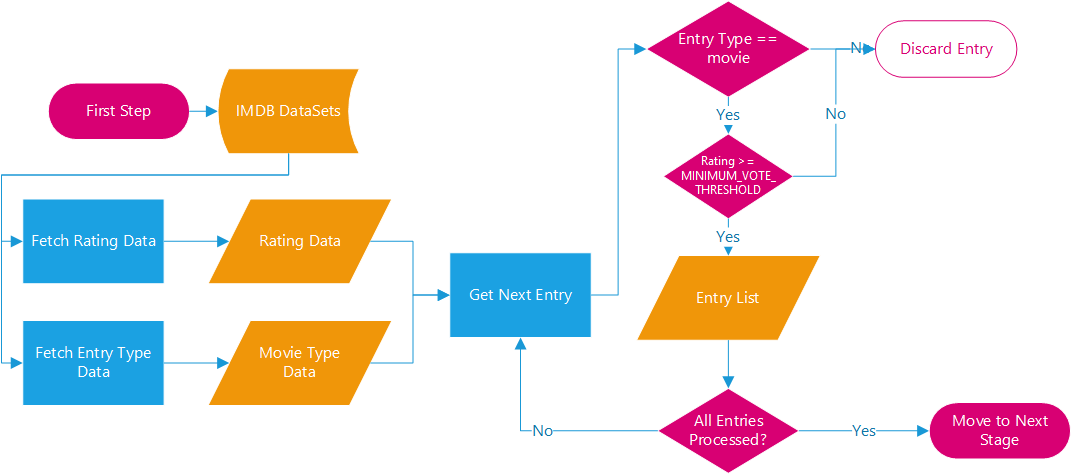
\includegraphics[width=150mm]{Chapters/5 - Architecture/Import/Images/imdb_flowchart.png}
  \caption{Διάγραμμα ροής δεδομένων από IMDB}
  \label{flowchart:imdbImport}
\end{figure}
\subsection{Βήμα 2ο - Δεδομένα από TMDb}
Στο 2ο βήμα αφού έχουμε τα δεδομένα που χρειάζονται από το πρώτο, δημιουργεί και προγραμματίζει για εκτέλεση ασύγχρονα ερωτήματα ζητώντας πλήρη δεδομένα ταινιών για κάθε αναγνωριστικό ταινίας που έχουμε στην υπηρεσία TMDb. 

Ο στόχος δεν είναι μόνο η απόκτηση δεδομένων ταινιών αλλά και συντελεστών, εταιριών και χωρών παραγωγής, και ειδών ταινιών, συνεπώς αφού πάρει τα δεδομένα ταινιών θα χρονοδρομολογήσει και άλλα ασύγχρονα ερωτήματα στην εν λόγω υπηρεσία για να πάρει και τα υπόλοιπα δεδομένα. 

Αφού τελειώσει αυτή η διαδικασία, συσχετίζει όλα τα δεδομένα μεταξύ τους και τα εισάγει στην βάση δεδομένων για περαιτέρω επεξεργασία από κάποιο άλλο σύστημα. 
\begin{figure}[h]
  \centering
  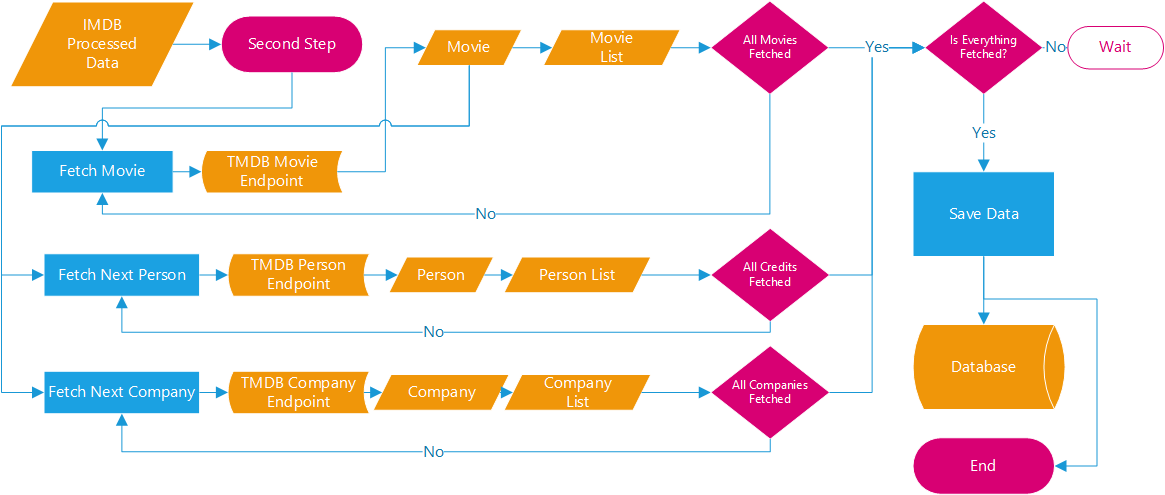
\includegraphics[width=150mm]{Chapters/5 - Architecture/Import/Images/tmdb_flowchart.png}
  \caption{Διάγραμμα ροής δεδομένων από TMDb}
  \label{flowchart:tmdbImport}
\end{figure}
\section{Σύστημα επεξεργασίας δεδομένων}
Ο Ρόλος του Συστήματος επεξεργασίας δεδομένων είναι να πάρει τα ανεπεξέργαστα δεδομένα από την βάση δεδομένων και να δημιουργήσει σχέσεις μεταξύ τους κατηγοριοποιώντας τα. Η Εφαρμογή προσφέρει δεδομένα ανά 4 κατηγορίες, και παράλληλα για κάθε κατηγορία ανά χρονολογική περίοδο. Η κατηγοριοποίηση είναι βασισμένη στα παρακάτω στοιχεία:
\begin{itemize}
    \item Στοιχεία ανά χώρα παραγωγής
    \item Στοιχεία ανά εταιρία παραγωγής
    \item Στοιχεία ανά συντελεστή - ξεχωριστά ανά ηθοποιό, συγγραφέα, σκηνοθέτη και παραγωγό
    \item Στοιχεία ανά είδος ταινίας
\end{itemize}

Η κάθε κατηγορία περιέχει στοιχεία για
την ταινία με την μεγαλύτερή αξιολόγηση, 
την ταινία με την χαμηλότερη αξιολόγηση, 
την μέση βαθμολογία ταινιών για αυτήν την κατηγορία, 
τις ταινίες με τα μεγαλύτερα και τα μικρότερα έσοδα και έξοδα, 
τα μέσα έξοδα / έσοδα ταινιών, 
τον πιο δημοφιλή και λιγότερο δημοφιλή ηθοποιό (ή συμπρωταγωνιστή αν η κατηγορία είναι ανά συντελεστή -- ηθοποιό), 
παραγωγό (η συμπαραγωγό αν η κατηγορία είναι ανά συντελεστή -- παραγωγό), 
σκηνοθέτη (η συν-σκηνοθέτη αν η κατηγορία είναι ανά συντελεστή -- σκηνοθέτη) και 
συγγραφέα (ή συν-συγγραφέα αν η κατηγορία είναι ανά συντελεστή -- συγγραφέα), 
την πιο δημοφιλή και λιγότερο δημοφιλή χώρα παραγωγής (η συμπαραγωγής αν η κατηγορία είναι ανά χώρα παραγωγής), 
την πιο δημοφιλή και λιγότερο δημοφιλή εταιρία παραγωγής (ή συμπαραγωγής αν η κατηγορία είναι ανά εταιρία παραγωγής) κ.α
όπως φαίνονται στο σχήμα ~\ref{model:movieinsights}.

\begin{figure}[p]
    \vspace*{-1cm}
    \hspace*{-1cm}
    \makebox[\linewidth]{
        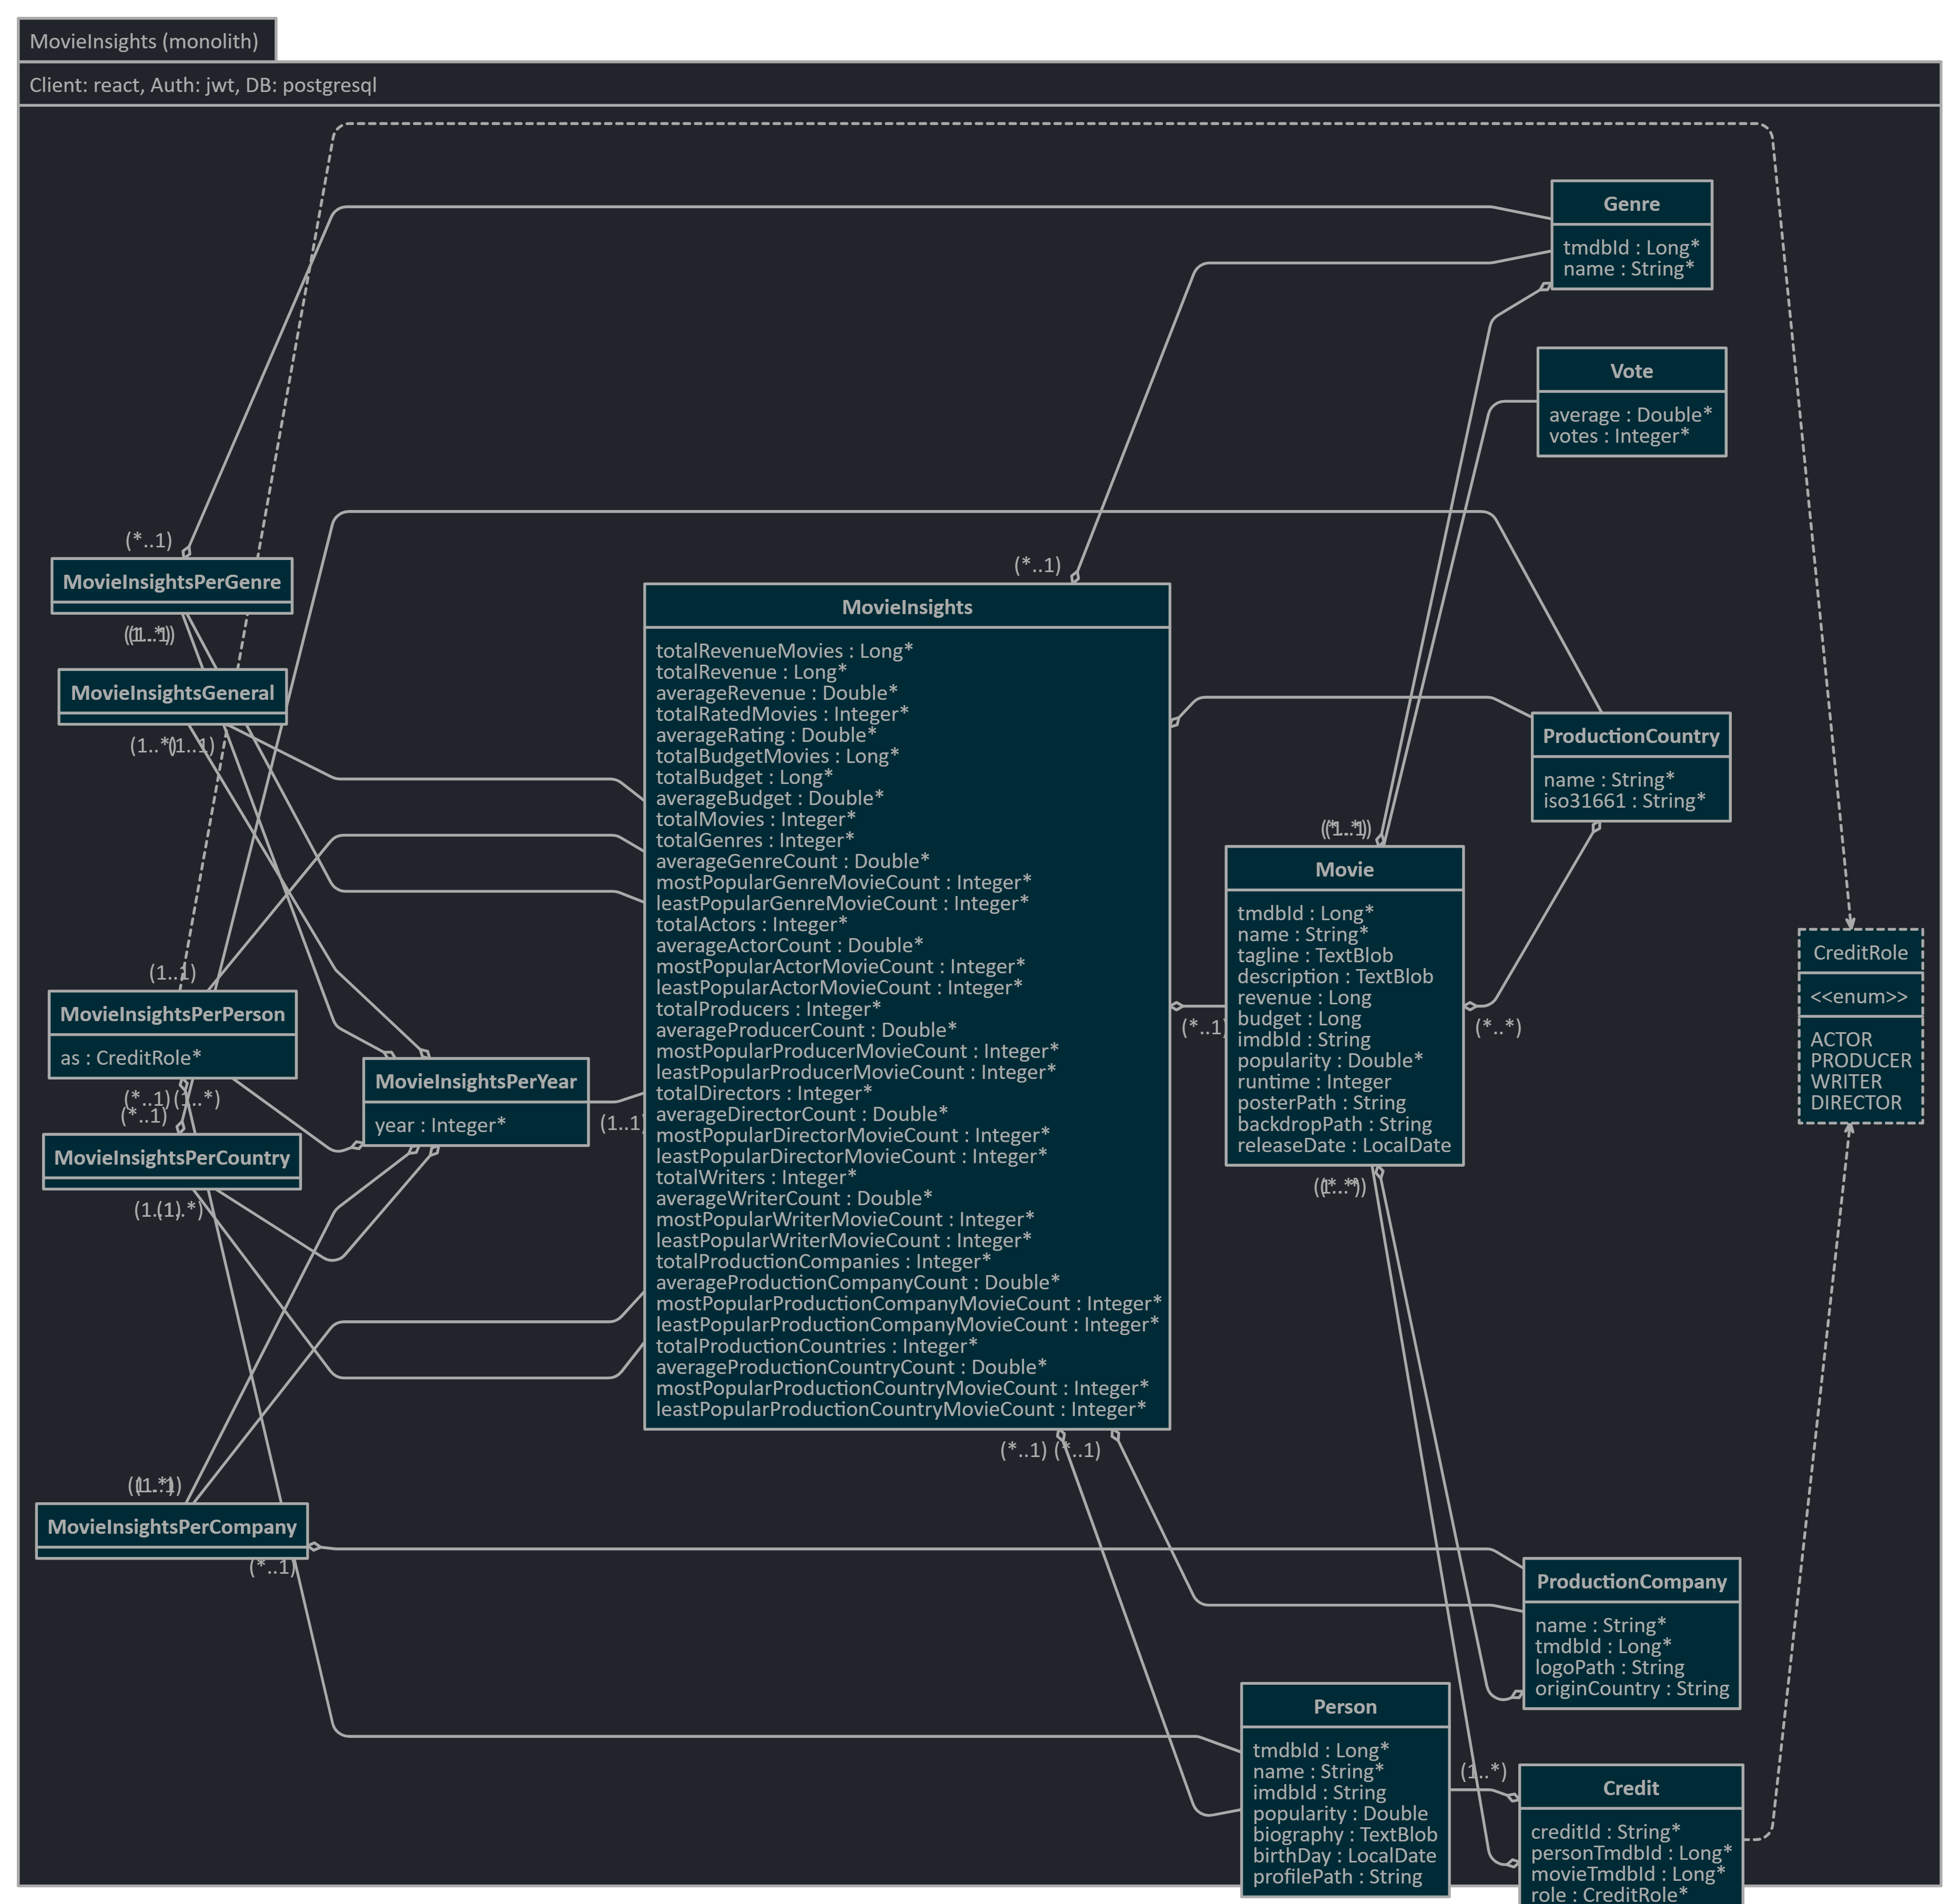
\includegraphics[width=1.4\linewidth]{Chapters/5 - Architecture/MovieInsights/Images/jhipster-jdl (2).png}
    }
   \caption{Μοντελο MovieInsights}
   \label{model:movieinsights}
\end{figure}

Η επεξεργασία των δεδομένων μπορούσε να γίνει είτε στο κομμάτι της βάσης δεδομένων με SQL είτε στο κομμάτι του Server με την Java. Ο πιο αποδοτικός τρόπος είναι να γίνει στην βάση δεδομένων με την SQL καθώς υπάρχουν διάφορα συστήματα βελτιστοποίησης τα οποία επιτρέπουν την επεξεργασία των δεδομένων αποδοτικά και γρήγορα, αλλά σε αυτήν την πτυχιακή προτιμήθηκε η Java για λόγους απλότητας.

Το σύστημα επεξεργασίας χωρίζεται σε 3 διαφορετικά κομμάτια. Το πρώτο κομμάτι συλλέγει και κατηγοριοποιεί τα δεδομένα. Το δεύτερο κομμάτι υπολογίζει τα μέγιστα τα ελάχιστα και τους μέσους των δεδομένων. Το τρίτο
κομμάτι μετατρέπει τα δεδομένα σε μια φιλική προς τη βάση δεδομένων μορφή και τα αποθηκεύει.

\subsection{Βήμα 1 - Κατηγοριοποίηση δεδομένων}
\begin{figure}[H]
    \begin{javacode}
    categories = new HashMap<>();
    getMovieInsights(long id, BaseWrapper<?> o) {
        if (categories.containsKey(id)) {
            return categoriess.get(id);
        }
        IMovieInsightsWrapper wrapper = createMovieInsightsWrapper(o);
        categories.put(id,wrapper);
        return wrapper;
    }
    getMovieInsightObjectsOptimized(Movie movie) {
     // return set of getMovieInsights(...)
    }
    categorizeData(Movie movie) {
        Set<IMovieInsightsWrapper> miSet = getMovieInsightObjectsOptimized(movie);
        miSet.forEach(wrapper -> {
            wrapper.submitMovie(movie);
        });
    }
    Lists
      .partition(dto.movies, 1000)
      .forEach(chunk -> {
         chunk.forEach(this::categorizeData);
      });
    \end{javacode}
    \caption{Σειριακή κατηγοριοποίηση με HashMap}
   \label{code:categorieSerialWithHM}
\end{figure}
Ο Αλγόριθμός κατηγοριοποίησης συλλέγει τα δεδομένα, τα προσθέτει στις ανάλογες κατηγορίες, δημιουργεί τις κατηγορίες αν δεν υπάρχουν, και ετοιμάζει τα δεδομένα για τον τελικό υπολογισμό.

Υπήρξαν πολλές αναθεωρήσεις του αλγορίθμου μέχρι την τελική του έκδοση. Οι περισσότερες αφορούσαν βελτιστοποιήσεις απόδοσης. 

Ο Αρχικός κώδικας (βλ σχήμα: \ref{code:categorieSerialWithHM}) ήταν αρκετά απλός. Είχε HashMaps για την αποθήκευση των δεδομένων ανά κατηγορία, και γινόταν συνεχώς έλεγχοι για το αν υπήρχαν τα δεδομένα. Αν όχι τα δημιουργούσε αλλιώς τα μορφοποιούσε.

Αρχικά ο κώδικας έτρεχε σειριακά, καθώς όμως αυξανόταν τα δεδομένα, ανέβαινε εκθετικά και ο χρόνος κατηγοριοποίησης τους. Για παράδειγμα για 1000 ταινίες μαζί με τους συντελεστές, τις εταιρίες και χώρες παραγωγής και τα είδη των ταινιών τους, έκανε 25 λεπτά για την ολοκλήρωση της κατηγοριοποίησης. Για 5000 ταινίες έκανε πάνω από 8 ώρες. 

Ο κώδικας ξαναγράφτηκε (βλ σχήμα: \ref{code:categorieParallelWithCHM}) για να τρέχει με παραλληλισμό. Έτσι κάποια βασικά στοιχεία άλλαξαν, όπως τα HashMaps έγιναν ConcurrentHashMaps και κάποια άλλα κομμάτια έγιναν Synchronize για να υπάρχει Thread Safety. Το αποτέλεσμα αυτών των αλλαγών ήταν η κατηγοριοποίηση 8000 ταινιών, συνυπολογίζοντας και τα λοιπά σχετικά στοιχεία, να ολοκληρώνεται εντός 25 λεπτών.

\begin{figure}[h]
    \begin{javacode}
    categories = new ConcurrentHashMap<>();
    categorizeData(Movie movie) { // ...
        miSet.parallelStream().forEach // ...
    }
    Lists
      // ...
         chunk
            .parallelStream().forEach // ...
      
    \end{javacode}
    \caption{Παράλληλης κατηγοριοποίηση με ConcurrentHashMap}
   \label{code:categorieParallelWithCHM}
\end{figure}

Στην πορεία εμφανίστηκε ένα πρόβλημα απόδοσης, το οποίο δεν ήταν ορατό κατά την πρώτη υλοποίηση, και το οποίο αφορούσε τα HashMaps.
Ενώ δίνουν με μεγάλη ευκολία, είναι στην ουσία ένα Indexer για την αποθήκευση key-value pairs, έχουν μεγάλο performance-pentalty όταν αρχίζει και μεγαλώνει ο όγκος των ανατεθειμένων δεδομένων και το πρόβλημα μεγεθύνεται ακόμα πιο πολύ όταν είναι και ConcurrentHashMaps λόγω των ελέγχων που γίνονται για το Thread Safety. Ένα δείγμα 30000 ταινιών έκανε πάνω από 4.5 ώρες για να κατηγοριοποιήθει.

Κάτι έπρεπε να αντικαταστήσει τα HashMaps. Στην τελική έκδοση του αλγόριθμου (βλ σχήμα: \ref{code:categorieParallelWithArr}) τα HashMaps αντικαταστάθηκαν με τα Native Arrays. Η επιλογή αυτή είχε ιδιαιτέρως θετικό αντίκτυπο στην ταχύτητα της κατηγοριοποίησης αλλά μεγάλωσε η πολυπλοκότητα διαχείρισης των δεδομένων.
Συγκριτικά με τη χρήση ConcurrentHashMaps, όπου η κατηγοριοποίηση 30.000 ταινιών εκτελούνταν σε 4,5 ώρες, ο ανανεωμένος αλγόριθμος κατηγοριοποίησε 30000 ταινίες σε μόλις 8 λεπτά. 

\begin{figure}[h]
    \begin{javacode}
    creditsArray = new MovieInsightsPersonWrapper[dto.maxPersonId][CreditRole.getSize()];
    companiesArray = new MovieInsightsCompanyWrapper[dto.maxCompanyId];
    countriesArray = new MovieInsightsCountryWrapper[dto.maxCountryId];
    genresArray = new MovieInsightsGenreWrapper[dto.maxGenreId];
    
    getMovieInsights(long id, BaseWrapper<?> o, IMovieInsightsWrapper[] array) {
        synchronized (array) {
            IMovieInsightsWrapper wrapper;
            if ((wrapper = array[(int) id]) == null) {
                array[(int) id] = wrapper = createMovieInsightsWrapper(o);
            }
            return wrapper;
        }
    }
    \end{javacode}
    \caption{Παράλληλη κατηγοριοποίηση με Arrays}
   \label{code:categorieParallelWithArr}
\end{figure}
Ο αλγόριθμος λοιπόν κατηγοριοποιεί τα δεδομένα όπως φαίνεται στο σχήμα \ref{flowchart:categorizeData} και αφού τελειώσει προχωράει στο βήμα 2 του υπολογισμού των δεδομένων.
\begin{figure}[H]
  \centering
  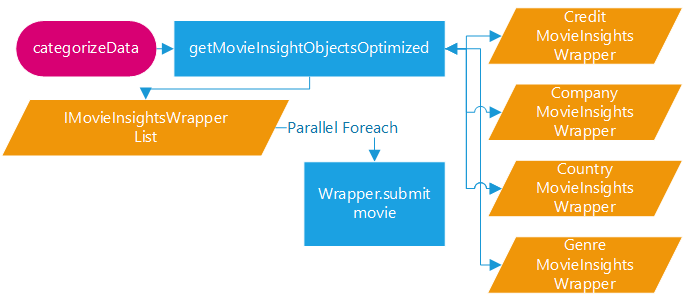
\includegraphics[width=150mm]{Chapters/5 - Architecture/MovieInsights/Images/categorizeData.png}
  \caption{Διάγραμμα ροής κατηγοριοποίησης δεδομένων}
  \label{flowchart:categorizeData}
\end{figure}
\subsection{Βήμα 2 - Υπολογισμός  δεδομένων}

Επιλέγοντας την γλώσσα προγραμματισμού Java για τον υπολογισμό των δεδομένων και επικεντρώνοντας όλες τις βελτιστοποιήσεις στο κομμάτι τις απόδοσης, δημιουργήθηκε ένα νέο πρόβλημα. Επειδή υπάρχουν διπλότυπα δεδομένα λόγω της φύσης της δομής της πτυχιακής, η παρούσα υλοποίηση δεν είναι καθόλου βελτιστοποιημένη για την χρήση μνήμης RAM. Στο πέρας του πρώτο βήματος με δεδομένα 30000 ταινιών κατηγοριοποιημένα, η χρήση μνήμης ξεπερνάει τα 25 GB. Έχοντάς αυτό σαν δεδομένο ο αλγόριθμος υπολογισμού των δεδομένων εκτός από αποδοτικός ως προς την ταχύτητα θα έπρεπε να είναι τουλάχιστον και αποδοτικός ως προς την χρήση μνήμης.

Η αρχική προσέγγιση ήταν ο υπολογισμός των δεδομένων σε κάποια DTO με σκοπό ύστερα την δημιουργία Managed Entities του Hibernate, για να μπορέσουν να αποθηκευτούν στην βάση δεδομένων. Με αυτόν τον τρόπο όμως θα είχαμε ξανά το φαινόμενο των διπλότυπων και θα ξοδεύαμε ακόμα περισσότερη μνήμη καθώς η πλειοψηφία των δεδομένων είναι Native Ints, Longs και Doubles και όχι τόσο Reference Types. Η προσέγγιση που επιλέχτηκε ήταν η δημιουργία ενός Wrapper που κληρονομεί από το Maanaged Entity του Hibernate, κάνοντας και το Wrapper, Managed Entity. Με λίγες ρυθμίσεις πλέον το Wrapper μπορεί να σταλεί απευθείας στον Hibernate για να αποθηκευτεί στην βάση δεδομένων χωρίς να χρειαστεί η δημιουργία κάποιου άλλου Managed Entity.

Για αυτόν τον λόγο ο αλγόριθμος της επεξεργασίας δεδομένων μεταφέρθηκε μέσα σε αυτό το Wrapper έτσι ώστε να μπορεί να τρέξει μετά το πέρας της κατηγοριοποίησης αποδοτικά. Βλέποντας πίσω στο σχήμα(\ref{code:categorieParallelWithCHM}) είναι εμφανές ότι αποστέλλεται μια ταινία στον Wrapper για περαιτέρω επεξεργασία. 

Για να βελτιστοποιηθεί ακόμα περισσότερο στο βήμα της κατηγοριοποίησης ο Wrapper εκτελεί όσους υπολογισμούς μπορεί, που δεν χρειάζονται τα συνολικά δεδομένα για να υπολογιστούν, αλλά μόνο τα υπάρχοντα κάθε φορά σε κάθε submit.

Τα δεδομένα που υπολογίζονται σε κάθε submit είναι οι ταινίες με την μεγαλύτερη και χαμηλότερη βαθμολογία καθώς και η μέση βαθμολογία ταινιών για κάθε κατηγορία και οι ταινίες με τα μεγαλύτερα και χαμηλότερα έσοδα/έξοδα καθώς και τα μέσα έσοδα/έξοδα για κάθε κατηγορία. Τα υπόλοιπα δεδομένα υποβάλλονται και αποθηκεύονται σε HashMaps για τον τελικό υπολογισμό.

Ένα πρόβλημα που αντιμετωπίστηκε στον υπολογισμό της ταινίας με την μεγαλύτερη βαθμολογία ήταν η ακρίβεια της βαθμολογίας. Για παράδειγμα δεν είναι το ίδιο να υπάρχει μια ταινία με βαθμολογία 9.0 και 10.000 ψήφους και μια άλλη ταινία με βαθμολογία 9.0 και 200.000 βαθμολογίες. Όπως επίσης είναι πιο αξιόπιστη μια βαθμολογία για παράδειγμα 8.5 με 2.000.000 ψήφους από ότι μια βαθμολογία 9.0 με 100.000 ψήφους. 

Για την επίλυση αυτού του προβλήματος χρησιμοποιήθηκε ένας πολύ απλός αλγόριθμος βάρους $rating * \log_2(voteCount)$, έτσι ώστε να υπολογίζονται και οι ψήφοι και να βγαίνει ενα "σκορ" ταινίας το οποιο θα συγκρίνεται με τα άλλα "σκορ" ταινιών έτσι ώστε να υπολογίζεται η με μεγαλύτερη ακρίβεια ποια ταινία είχε την μεγαλύτερη βαθμολογία.
\begin{figure}[h]
    \begin{javacode}
double calculateScore(Vote vote, boolean high) {
    return getScore(vote.getAverage(), vote.getVotes(), high, 2);
}
double getScore(double value, double weight, boolean high, int base) {
    double weightLog = Math.log(weight) / Math.log(base);
    return high ? value * weightLog : value / weightLog;
}
    \end{javacode}
    \caption{Αλγόριθμος Βάρους Βαθμολογιών}
   \label{code:logarithmicScore}
\end{figure}

Με τον παραπάνω αλγόριθμο σαν βάση, ο Αλγόριθμος υπολογισμού των ταινιών με την μεγαλύτερη και χαμηλότερη βαθμολογία καθώς και της μέσης βαθμολογίας έχει διαμορφωθεί όπως φαίνεται στο σχήμα ~\ref{code:ratingCalculation}. Αρχικά γίνεται έλεγχος αν οι ψήφοι της βαθμολογίας της εν λόγω ταινίας είναι περισσότεροι ή ίσοι με την τιμή της σταθεράς {\it MINIMUM\_VOTES\_THRESHOLD}. Αν δεν είναι, η ταινία εξαιρείται από αυτόν τον υπολογισμό. Αλλιώς προστίθεται η βαθμολογία της ταινίας σε μια μεταβλητή που κρατάει το άθροισμά όλων των βαθμολογιών και αυξάνεται η μεταβλητή που κρατάει και πόσες ταινίες έχουν υποβάλει τις βαθμολογίες τους, για να υπολογιστεί αργότερα η μέση βαθμολογία ταινιών. Ύστερα αν δεν υπάρχει ήδη ταινία με την μεγαλύτερη η χαμηλότερη βαθμολογία τοποθετείται αυτή για την οποία γίνεται ο έλεγχος αυτήν την χρονική στιγμή, αλλιώς γίνεται έλεγχος αν αυτή η ταινία έχει μεγαλύτερη / μικρότερη βαθμολογία από την ανάλογη υπάρχουσα και ορίζεται αυτή στην θέση της σε περίπτωση που πληροί της προϋποθέσεις.

\begin{figure}[h]
    \begin{javacode}
void submitRating(Movie movie) {
    if (movie.getVote().getVotes() >= Constants.MINIMUM_VOTES_THRESHOLD) {
        synchronized (voteLock) {
            Vote vote = movie.getVote();
            totalVoteAverage += vote.getAverage();
            setTotalRatedMovies(getTotalRatedMovies() + 1);
            if (getHighestRatedMovie() == null) {
                setHighestRatedMovie(movie);
            } else {
                setHighestRatedMovie(calculateVote(calculateScore(getHighestRatedMovie().getVote(), true), getHighestRatedMovie(),calculateScore(movie.getVote(), true),movie,(current, challenger) -> current < challenger));
            }
            if (getLowestRatedMovie() == null) {
                setLowestRatedMovie(movie);
            } else {
                setLowestRatedMovie(calculateVote( getLowestRatedMovie().getVote().getAverage(),getLowestRatedMovie(), movie.getVote().getAverage(),movie,(current, challenger) -> current > challenger));
            }
        }
    }
}   
    \end{javacode}
    \caption{Αλγόριθμος Υπολογισμού Βαθμολογιών}
   \label{code:ratingCalculation}
\end{figure}

Ο υπολογισμοί των ταινιών με τα μεγαλύτερα, μικρότερα και μέσα έσοδα / έξοδα γίνεται με έναν πολύ παρόμοιο τρόπο όπως των βαθμολογιών των ταινιών, χωρίς βέβαια να χρησιμοποιείται ο αλγόριθμος βάρους.

Ο υπολογισμός των υπόλοιπων δεδομένων γίνεται μετά το πέρας του βήματος της κατηγοριοποίησης. Για να γίνει πιο εύκολος ο υπολογισμός, αντί να υποβάλλονται τα δεδομένα ως έχουν έχουν δημιουργηθεί Wrappers γύρο από αυτά για την προσθήκη επιπρόσθετων δεδομένων και λειτουργιών που καθιστούν τον υπολογισμό των δεδομένων πιο εύκολο. Για παράδειγμα ένα αντικείμενο τύπου Genre έχει το ανάλογο GenreWrapper, όπως επίσης και ένα αντικείμενο τύπου Person έχει ανάλογα ActorWrapper, DirectorWrapper, ProducerWrapper και WritterWrapper για κάθε κατηγορία ατόμου που υποστηρίζεται από την εφαρμογή. Σε αυτά τα Wrappers υπάρχουν δεδομένα όπως ο αριθμός ταινιών που συμμετέχουν αυτά τα Wrappers για αυτήν την κατηγορία, οι ταινίες οι ίδιες, και υπάρχουν και λειτουργίες σύγκρισης (Comparators) μεταξύ ίδιων Wrappers χρησιμοποιώντας αυτά τα παραπάνω δεδομένα.

Όταν γίνεται η υποβολή δημιουργείται αρχικά ένα Wrapper προσθέτοντάς μεταδεδομένα χωρίς να ελεγχθεί αν υπάρχει ήδη Wrapper που να αναφέρεται στο ίδιο αντικείμενο, αποθηκευμένο στο ανάλογο HashMap οπως φαίνεται στο σχήμα \ref{code:submitGenre}, στην σειρά 5 για την υποβολή δεδομένων ειδών ταινιών.
\begin{figure}[h]
    \begin{javacode}
void submitGenres(Movie movie) {
    AtomicBoolean hasIncreased = new AtomicBoolean(false);
    movie.getGenres().parallelStream().filter(Objects::nonNull).forEach(genre -> {
        calculateTotals(genreTotals, hasIncreased);
        submit(new GenreWrapper(genre, processor.getMovieCount(genre)), genres, movie, genre);
    });
}
    \end{javacode}
    \caption{Αλγόριθμος Υποβολής Δεδομένων Είδους Ταινίας}
    \label{code:submitGenre}
\end{figure}

Στην γενικευμένη συνάρτηση submit πάραυτα γίνεται εκεί ο έλεγχος για την ύπαρξη του ανάλογου Wrapper, και αν υπάρχει απλά αγνοεί το νέο Wrapper και αλλάζει το υπάρχων χρησιμοποιώντας τα στοιχεία του νεου, αλλιώς τοποθετεί το δημιουργημένο Wrapper στο ανάλογο HashMap όπως φαίνεται στο σχήμα \ref{code:submit}.

\begin{figure}[h]
    \begin{javacode}
<T extends IdentifiedEntity, W extends BaseWrapper<T>> void submit(W wrapper, Map<Long, W> objMap, Movie movie, T obj) {
    W wrapper2;
    synchronized (objMap) {
        if ((wrapper2 = objMap.putIfAbsent(obj.getId(), wrapper)) == null) {
            wrapper2 = wrapper;
        }
    }
    wrapper2.movies.add(movie);
    wrapper2.count++;
}
    \end{javacode}
    \caption{Αλγόριθμος Γενικευμένης υποβολής δεδομένων}
    \label{code:submit}
\end{figure}

Επιπρόσθετα για τον υπολογισμό αυτών των δεδομένων χρησιμοποιείται μια βοηθητική γενικευμένη κλάση Total, η οποία κρατάει τα στοιχεία για τα μέγιστα, ελάχιστα και μέσα αυτών των δεδομένων. 

Μετά το πέρας της συλλογής και της κατηγοριοποίησης των δεδομένων, το κάθε MovieInsights Wrapper ξεχωριστά θα υπολογίσει τα υπόλοιπα δεδομένα για το ίδιο αλλά και για κάθε εξαρτώμενο Wrapper από αυτό, που στην συγκεκριμένη περίπτωση τα εξαρτώμενα Wrappers, είναι οι κατηγορίες ανά χρόνο.

Για κάθε διαφορετικό Wrapper HashMap θα υπολογιστούν τα μέγιστα και τα ελάχιστα χρησιμοποιώντας τις συναρτήσεις σύγκρισης που υπάρχουν μέσα στα Wrappers, και τα δεδομένα που περιέχουν τα μέγιστα και τα ελάχιστα θα υποβληθούν στα αντικείμενα της βοηθητικής κλάσης Total για την ανάκτηση τους αργότερα, όπως φαίνεται στα σχήματα \ref{code:calculateChildInsights} και \ref{code:getWrapperBasedOnComparator}.

\begin{figure}[h]
    \begin{javacode}
<W extends BaseWrapper<WE>, WE> void calculateChildInsights(Map<Long, W> map, Comparator<? super W> comparator, Total<WE> totals) {
    Optional<W> mostPopularEntryResult = getWrapperBasedOnComparator(map, comparator.reversed());
    mostPopularEntryResult.ifPresent(totals::submitMostPopular);
    Optional<W> leastPopularEntryResult = getWrapperBasedOnComparator(map, comparator);
    leastPopularEntryResult.ifPresent(totals::submitLeastPopular);
    totals.setTotalEntities(map.size());
}
    \end{javacode}
    \caption{Γενικευμένος Αλγόριθμος υπολογισμού μέγιστων και ελάχιστων δεδομένων}
    \label{code:calculateChildInsights}
\end{figure}
\begin{figure}[h]
    \begin{javacode}
private <W extends BaseWrapper<EW>, EW> Optional<W> getWrapperBasedOnComparator(Map<Long, W> wrapperMap, Comparator<? super W> comparator) {
    return wrapperMap.values().parallelStream().sorted(comparator).filter(e -> (slave ? master.getCategory() : getCategory()) != e.category || e.object != (slave ? master.getSource().object : source.object)).findFirst();
}
    \end{javacode}
    \caption{Γενικευμένος Αλγόριθμος ανάκτησης Wrapper απο ενα HashMap με βάση αλγόριθμο σύγκρισης}
    \label{code:getWrapperBasedOnComparator}
\end{figure}

Τέλος όλα τα δεδομένα αποθηκεύονται στα πεδία της κληρονομουμένης κλάσης MovieInsights, ανακτώντας τα δεδομένα από τα αντικείμενα της βοηθητικής κλάσης Total.

% \begin{figure}[h]
%     \begin{javacode}
% void submitRevenue(Movie movie) {
%     if (movie.getRevenue() >= Constants.MINIMUM_REVENUE_THRESHOLD) {
%         synchronized (revenueLock) {
%             setTotalRevenue(getTotalRevenue() + movie.getRevenue());
%             setTotalRevenueMovies(getTotalRevenueMovies() + 1);
%             if (getHighestRevenueMovie() == null) {
%                 setHighestRevenueMovie(movie);
%             } else {
%                 if (getHighestRevenueMovie().getRevenue() < movie.getRevenue()) {
%                     setHighestRevenueMovie(movie);
%                 } else if (getHighestRevenueMovie().getRevenue().equals(movie.getRevenue()) && movie.getPopularity() > getHighestRevenueMovie().getPopularity()) {
%                     setHighestRevenueMovie(movie);
%                 }
%             }
%             if (getLowestRevenueMovie() == null) {
%                 setLowestRevenueMovie(movie);
%             } else {
%                 if (getLowestRevenueMovie().getRevenue() > movie.getRevenue()) {
%                     setLowestRevenueMovie(movie);
%                 } else if (getLowestRevenueMovie().getRevenue().equals(movie.getRevenue()) && movie.getPopularity() > getLowestRevenueMovie().getPopularity()) {
%                     setLowestRevenueMovie(movie);
%                 }
%             }
%         }
%     }
% }    
%     \end{javacode}
%     \caption{Αλγόριθμος Υπολογισμού Εσόδων}
%   \label{code:revenueCalculation}
% \end{figure}
% \begin{figure}[h]
%     \begin{javacode}
% void submitBudget(Movie movie) {
%     if (movie.getBudget() >= Constants.MINIMUM_BUDGET_THRESHOLD) {
%         synchronized (budgetLock) {
%             setTotalBudget(getTotalBudget() + movie.getBudget());
%             setTotalBudgetMovies(getTotalBudgetMovies() + 1);
%             if (getHighestBudgetMovie() == null) {
%                 setHighestBudgetMovie(movie);
%             } else {
%                 if (getHighestBudgetMovie().getBudget() < movie.getBudget()) {
%                     setHighestBudgetMovie(movie);
%                 } else if (getHighestBudgetMovie().getBudget().equals(movie.getBudget()) && movie.getPopularity() > getHighestBudgetMovie().getPopularity()) {
%                     setHighestBudgetMovie(movie);
%                 }
%             }
%             if (getLowestBudgetMovie() == null) {
%                 setLowestBudgetMovie(movie);
%             } else {
%                 if (getLowestBudgetMovie().getBudget() > movie.getBudget()) {
%                     setLowestBudgetMovie(movie);
%                 } else if (getLowestBudgetMovie().getBudget().equals(movie.getBudget()) && movie.getPopularity() > getLowestBudgetMovie().getPopularity()) {
%                     setLowestBudgetMovie(movie);
%                 }
%             }
%         }
%     }
% }
%     \end{javacode}
%     \caption{Αλγόριθμος Υπολογισμού Εξόδων}
%     \label{code:budgetCalculation}
% \end{figure}
% \begin{javacode*}{frame=none,fontsize=\small,linenos=false}
% void calculateChildInsights(Map<Long, W> map, Comparator<? super W> comparator, Total<WE> totals)
% \end{javacode*}

\subsection{Βήμα 3 - Αποθήκευση δεδομένων}
Έχοντάς συλλέξει, κατηγοριοποιήσει και υπολογίσει όλα τα απαραίτητα δεδομένα, τα δεδομένα αυτά με ελάχιστες μετατροπές στέλνονται στον Hibernate για να αποθηκευτούν στην βάση δεδομένων έτσι ώστε να τεθεί η εφαρμογή σε κατάσταση ετοιμότητας. 

Για την αποθήκευση δεδομένων δημιουργείται μια νέα "συναλλαγή". Η συναλλαγή αυτή βεβαιώνει ότι αν κάποιο από τα δεδομένα αυτά δεν μπορούσε για οποιονδήποτε λόγω να αποθηκευτεί στην βάση δεδομένων, να ακυρωθεί όλη αυτή η διαδικασία και να τερματίσει η εφαρμογή με το ανάλογο μήνυμα σφάλματος, έτσι ώστε να μπορεί να επιλυθεί απο κάποιον διαχειριστή. Η αποθήκευση μερικών δεδομένων στην βάση δεδομένων θα είχε καταστροφικές συνέπειες στην λειτουργία της εφαρμογής. 

Μετά το πέρας της αποθήκευσης, γίνεται εκκαθάριση του Cache και ζητείται να γίνει και εκκαθάριση μνήμης από τον Garbage Collector το JVM, ώστε να ελευθερωθεί μνήμη για την καλύτερη λειτουργία της εφαρμογής. Πολλές φορές αυτό δεν είναι δυνατό ανάλογα με το JVM που χρησιμοποιείται και έτσι μετά την αρχικοποίηση στην περίπτωση που δεν υπάρχει διαθέσιμη μνήμη συστήνεται η επανεκκίνηση της εφαρμογής.


\section{Μηχανή Αναζήτησης}
Η μηχανή αναζήτησης είναι μια σημαντική υπηρεσία για την εφαρμογή και επιτρέπει στον χρήστη την αναζήτηση και αυτόματη συμπλήρωση της αναζήτησης ατόμων, εταιριών παραγωγής, χωρών παραγωγής και ειδών ταινιών. 

Η μηχανή αναζήτησης έχει την δυνατότητα να συνδεθεί σε μια εξωτερική βαση δεδομένων για την ανάκτηση δεδομένων είτε να χρησιμοποιήσει την εσωτερική της βάση δεδομένων. Για την βελτιστοποίηση της εμπειρίας του χρήστη η μηχανή αναζήτησης χρησιμοποιεί την δικιά της βάση δεδομένων, καθώς είναι πολύ πιο γρήγορη απο μια συμβατική SQL βάση δεδομένων, με το μειονέκτημα της διπλοτυπίας δεδομένων. 

Για περαιτέρω βελτιστοποίηση δημιουργήθηκαν ξεχωριστά Indices για την μηχανή αναζήτησης και ξεχωριστά Entities για την βάση δεδομένων. Έχοντάς ως κύρια πηγή της αλήθειας τα Entities της βάσης δεδομένων SQL, τα Indicies της μηχανής αναζήτησης έχουν τα λιγότερα δυνατά δεδομένα που χρειάζονται για την αναζήτηση, μειώνοντας σημαντικά τον απαιτούμενο χώρο αποθήκευσης.

Καθώς όμως τα δεδομένα δεν βρίσκονται σε μια μόνο βάση δεδομένων, χρειάζεται ο συγχρονισμός τους καθ όλη την λειτουργία της εφαρμογής. Αυτό γίνεται εύκολα καθώς τα δεδομένα που χρησιμοποιούνται στην αναζήτηση, αλλάζουν μόνο όταν τρέχει το σύστημα εισαγωγής δεδομένων και αυτό γίνεται μόνο στην εκκίνηση της εφαρμογής.

Πάραυτα καθώς η μηχανή αναζήτησης είναι ένα εξωτερικό σύστημα, όχι άμεσα επιβλεπόμενο απο την εφαρμογή, τα δεδομένα της βάσης δεδομένων της, μπορούν να αλλάξουν και να αλλοιωθούν ανά πάσα στιγμή. Για αυτόν τον λόγο έχει δημιουργηθεί μια υπηρεσία που οι αποκλειστικές αρμοδιότητες της είναι να συγχρονίζει τα δεδομένα της κύριας βάσης δεδομένων με την βάση δεδομένων της μηχανής αναζήτησης. Αυτή η υπηρεσία ενεργεί μια φορά στην εκκίνηση ακριβώς πριν τεθεί η εφαρμογή σε κατάσταση ετοιμότητας, και ενεργεί όταν ένας διαχειριστής το ζητήσει. 

Η Μηχανή Αναζήτησης πέρα απο τον συγχρονισμό δεδομένων επιτρέπει τον χρήστη να αναζητήσει κάτι, αλλα παράλληλα επιτρέπει και την αυτόματη συμπλήρωση. Για να λειτουργήσει η Αυτόματη συμπλήρωση όλα τα Indices έπρεπέ να ρυθμιστούν ανάλογα.

\begin{figure}[H]
    \begin{jsoncode}
{"analysis": {
  "filter": {
    "autocomplete_filter": {
      "type": "edge_ngram",
      "min_gram": 1,
      "max_gram": 40
    }
  },
  "analyzer": {
    "autocomplete_search": {
      "type": "custom",
      "tokenizer": "standard",
      "filter": ["lowercase"]
    },
    "autocomplete_index": {
      "type": "custom",
      "tokenizer": "standard",
      "filter": ["lowercase", "autocomplete_filter"]
    }
  }
}}
    \end{jsoncode}
    \caption{Ρυθμίσεις ενός Index της ElasticSearch}
   \label{config:es}
\end{figure}

Για να λειτουργήσει η αυτόματη συμπλήρωση κάθε λέξη και πρόταση μέσα σε αυτά τα Indices έπρεπε να χωριστεί σε ngrams. Όπως φαίνεται στο σχήμα \ref{config:es} στην σειρά 18, δηλώθηκε ενα φίλτρο το οποίο σπάει τις λέξεις και προτάσεις σε ngrams και ετσι επιτρέπει την ρύθμιση ενός πεδίου ενός Index για να μπορεί να αναζητηθεί με αυτόματη συμπλήρωση.

Το επόμενο βήμα ήταν να δηλωθούν τα πεδία στα Indices που θα έχουν τα φίλτρα του autocomplete, όπως φαίνεται στο σχήμα \ref{code:index}

\begin{figure}[h]
    \begin{javacode}
@MultiField(
    mainField = @Field(
        type = Text, 
        fielddata = true,
        analyzer = "autocomplete_index", 
        searchAnalyzer = "autocomplete_search"),
    otherFields = {@InnerField(suffix = "verbatim", type = Keyword)})
private String name;
    \end{javacode}
    \caption{Annotations ενός Index της ElasticSearch}
   \label{code:index}
\end{figure}

Με αυτόν τον τρόπο δηλώνονται τα Indices στον κώδικα με τις σωστές ρυθμίσεις, και η βιβλιοθήκη που χρησιμοποιήθηκε για να επικοινωνήσει με την ElasticSearch, Jest αρχικοποιεί τα Indices στην ElasticSearch και αφου προστεθούν δεδομένα απο τον συγχρονισμό των 2 βάσεων, η μηχανή αναζήτησης είναι έτοιμη για χρήση.

Καθώς όπως προαναφέρθηκε η ElasticSearch είναι ένα αυτόνομο σύστημα πρέπει να του δοθεί ενα ανάλογο Query που να μπορεί να το καταλάβει για να μπορέσει να σερβίρει τα δεδομένα. Αυτό το κάνει η υπηρεσία SearchService.

Όλα τα entities της εφαρμογής έχουν το ανάλογο Service για να επιτρέψουν την ανάκτηση, μορφοποιήση, δημιουργεία αλλα και διαγραφή των δεδομένων τους, γνωστό ως CRUD. Τα Entities που έχουν ανάλογα Indicies μοιράζονται τα ίδια Services για λόγους απλότητας και συγκέντρωσης των αρμοδιοτήτων σε ενα σημείο. 

Κάθε υπηρεσία ενός Entity που έχει παράλληλα και Index, κάνει εγγραφή στο SearchService κατα την εκκίνηση, έτσι ώστε οταν φτάσει η στιγμή που θα γίνει ένα ερώτημα αναζήτησης, το SearchService να γνωρίζει απο ποια Indices θα παρθούν τα δεδομένα. Το κάθε Service που γίνεται register ορίζει επίσης ένα Query. Με αυτόν τον τρόπο η μηχανή αναζήτησης δεν χρειάζεται να γνωρίζει τίποτα για τα Indices, απλά παίρνει τα ερωτήματα απο όλα τα Services που δηλώνουν Indices, τα συνδιάζει και τα στέλνει στην ElasticSearch. Οταν πάρει τα δεδομένα, τα αλλάζει μορφή και τα στέλνει στον Client σε μια διαφορετική μορφή για την βελτιστοποίηση του μεγέθους της απάντησης. 

Όταν γίνεται η αυτόματη συμπλήρωση, για κάθε γράμμα που πληκτρολογείται στον Client, γίνεται και ένα ερώτημα στον Server και στην Μηχανή Αναζήτησης. Είναι πολύ σημαντικό και η μηχανή αναζήτησης να σερβίρει τα δεδομένα πολύ γρήγορα, αλλα και ο Server να απαντάει πολύ γρήγορα. Πέρα απο την ταχύτητα που θα απαντάει ο Server, πρέπει επίσης η απάντηση να είναι μικρή έτσι ώστε πρώτον να εξοικονομεί δεδομένα απο clients οι οποίοι βρίσκονται σε Metered Connections, και να στέλνονται πιο γρήγορα τα αποτελέσματα σε Clients οι οποίοι έχουν χαμηλή ταχύτητα Internet.

Για παράδειγμα το αποτέλεσμα της αναζήτησης που επιστρέφει η μηχανή αναζήτησης όπως φαίνεται στο σχήμα \ref{result:es} έχει μέγεθος 420 bytes για ένα αποτέλεσμα με μέγεθος αποτελέσματος 232 bytes, σε αντίθεση με το αποτέλεσμα του SearchService όπως φαίνεται στο σχήμα \ref{result:ss} με μέγεθος 166 bytes, για ένα αποτέλεσμα με μέγεθος αποτελέσματος 123 bytes. Είναι εμφανές λοιπόν οτι με την βελτιστοποίηση το μέγεθος της απάντησης είναι πολύ μικρότερο.

\begin{figure}[H]
    \begin{jsoncode}
{
    "took": 23,
    "timed_out": false,
    "_shards": {
        "total": 1,
        "successful": 1,
        "skipped": 0,
        "failed": 0
    },
    "hits": {
        "total": 37470,
        "max_score": 846.1094,
        "hits": [{
            "_index": "person",
            "_type": "person",
            "_id": "323",
            "_score": 846.1094,
            "_source": {
                "popularity": 35.808,
                "name": "Some Person",
                "profilePath": "/cckcYc2v0yh1tc9QjRelptcOBko.jpg",
                "id": 323
            }
        }]
    }
}
    \end{jsoncode}
    \caption{Αποτέλεσμα αναζήτησης ElasticSearch}
   \label{result:es}
\end{figure}
\begin{figure}[H]
    \begin{jsoncode}
{
    "_": [{
        "e": [{
            "id": 323,
            "name": "Some Person",
            "popularity": 35.808,
            "profilePath": "/cckcYc2v0yh1tc9QjRelptcOBko.jpg"
        }],
        "i": "PERSON"
    }]
}
    \end{jsoncode}
    \caption{Αποτέλεσμα Αναζήτησης SearchService}
   \label{result:ss}
\end{figure}

\section{Client}
Πέρα απο τον Server όπως προαναφέρθηκε το 2ο μέρος της εφαρμογής είναι ο Client. Ο Client είναι το σύστημα που θα καταναλώσει τα δεδομένα απο τον Server και θα τα εμφανίσει με έναν ευκατανόητο τρόπο στον χρήστη. Ο Client δομήθηκε με την χρήση της βιβλιοθήκης React του CoreUI και του Redux Framework.

Η React είναι η κεντρική βιβλιοθήκη που χρησιμοποιήθηκε και όλα τα αλλα συστήματα αλληλεπιδρούν με αυτήν. Το Redux χρησιμοποιήθηκε για την διαχείρισή της κατάστασης της εφαρμογής και το CoreUI για τα γραφικά της. Πέρα απο αυτές τις κύριες τεχνολογίες χρησιμοποιήθηκε επίσης η βιβλιοθήκη Highcharts για τα γραφήματα, τα εικονίδια της βιβλιοθήκης CoreUI και FontAwesome, η βιβλιοθήκη lodash για την ευκολότερη διαχείρισή των Javascript objects, και κάποιες άλλες μικρότερες βιβλιοθήκες για την βελτίωση της αισθητικής του γραφικού περιβάλλοντος. 

Ο Client στην ουσία είναι μια Web εφαρμογή και αποτελείται απο 2 κομμάτια. Το πρώτο είναι το Dashboard, το οποίο εμφανίζει ολα τα δεδομένα που προσφέρει ο Server. Το δεύτερο κομμάτι είναι η σελίδα παρακολούθησης των στατιστικών των υπηρεσιών. Παραυτα η αρχιτεκτονική του Client είναι SPA, που σημαίνει οτι υπάρχει μόνο μια σελίδα και το περιεχόμενο της σελίδας αλλάζει με την γλώσσα JavaScript. 

Η React λειτουργεί με Components. Component είναι ενα στοιχείο το οποίο εμφανίζεται κάπου μεσα στην Web εφαρμογή. Η Συνολική εφαρμογή αποτελείται απο πολλά Components τα οποία συνδιάζονται και εμφανίζονται μαζί για να φανεί το τελικό αποτέλεσμα. Τα Component είναι ένας έξυπνος τρόπος δόμησης μιας Web Εφαρμογής καθώς μπορούν να ξανα χρησιμοποιηθούν σε πολλά μέρη της εφαρμογής. Με αυτόν τον τρόπο έχοντας ενα αρχείο για κάθε Component γίνεται πιο ξεκάθαρη η δομή μιας εφαρμογής και ο τρόπος που λειτουργεί το κάθε Component, και καθίσταται ευκολότερη η συντήρηση και αλλαγή κώδικα αλλα και η αντιμετώπιση σφαλμάτων. 

Η Βασική δομή αποτελείται απο το Header Component, το Router Component και το Footer Component όπως φαίνεται στο σχήμα \ref{wire:main}. Το Header αποτελείται απο μια εικόνα, το λογότυπο της εφαρμογής, στα αριστερά και ένα εικονίδιο με εικόνα ενα γρανάζι στα δεξιά το οποίο επιτρέπει την αλλαγή γλώσσας, την είσοδο στην εφαρμογή και σε περίπτωση που ο χρήστης είναι ήδη εξουσιοδοτημένος εναν σύνδεσμο στο πάνελ διαχείρισης. Το footer αναγράφει την ημερομηνία κατασκευής της εφαρμογής καθώς και το όνομα του δημιουργού στα αριστερά, και στα δεξιά αναγράφει τις κύριες τεχνολογίες που χρησιμοποιήθηκαν για να γίνει η εφαρμογή. Το Router απο την άλλη είναι μια περιοχή η οποία θα αλλάζει ανάλογα με το τι χρειάζεται να εμφανιστεί κάθε φορά.

\begin{figure}[h]
  \centering
  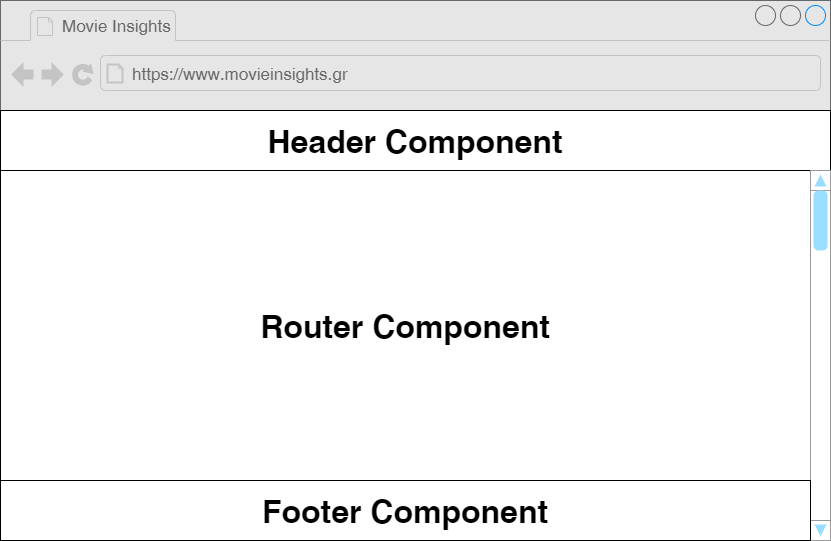
\includegraphics[width=145mm]{Chapters/5 - Architecture/Client/Images/main_struct.png}
  \caption{Βασική διάταξη Web εφαρμογής}
  \label{wire:main}
\end{figure}

Η εφαρμογή αυτή επίσης έχει Modules. Η ένοια Module στην React δεν υπάρχει σε αντιθεση με κάποιο αλλο Web Framework όπως η Angular, αλλα για αυτήν την εφαρμογή στην ουσία ορίζει μια λειτουργία και ομαδοποιεί ολα τα Components αυτής της λειτουργίας μαζί. 

Η αρχιτεκτονική του Router είναι δυναμική καθώς επιτρέπει κάθε module να ορίζει το δικο της Router με τα δικά του Routes. Υπάρχουν 2 ειδών Routes. Το πρώτο είναι το απλο Route που όταν αλλάζει η διεύθυνση στην γραμμή εισαγωγής διεύθυνσης σελίδας αλλάζει και το περιεχόμενο. Το δεύτερο ονομάζεται PrivateRoute και επιτρέπει την πρόσβαση στην δηλωμένη διεύθυνση μόνο αν ο χρήστης έχει κάνει Login, και είναι εξουσιοδοτημένος για να δεί αυτό που ζητάει. 

\subsection{Dashboard Module}
Το Dashboard είναι το κεντρικό Module της εφαρμογής, που φαίνεται και στην αρχική σελίδα και εμφανίζει μέσω του MIDashboard Component 4 διαφορετικά κομμάτια. Το πρώτο κομμάτι είναι η μπάρα αναζήτησης, το δεύτερο κομμάτι είναι ένας παγκόσμιος χάρτης, το τρίτο κομμάτι είναι στα δεξιά του χάρτη και αποτελείται από γραφήματα και συγκεντρωτικά στοιχεία και το τέταρτο και τελευταίο κομμάτι είναι τα κύρια δεδομένα της εφαρμογής όπως ο πιο δημοφιλής ηθοποιός, η ή ταινία με τα μεγαλύτερα έσοδα κ.λ.π όπως φαίνεται στο σχήμα \ref{wire:dashboard}.

\begin{figure}[H]
  \centering
  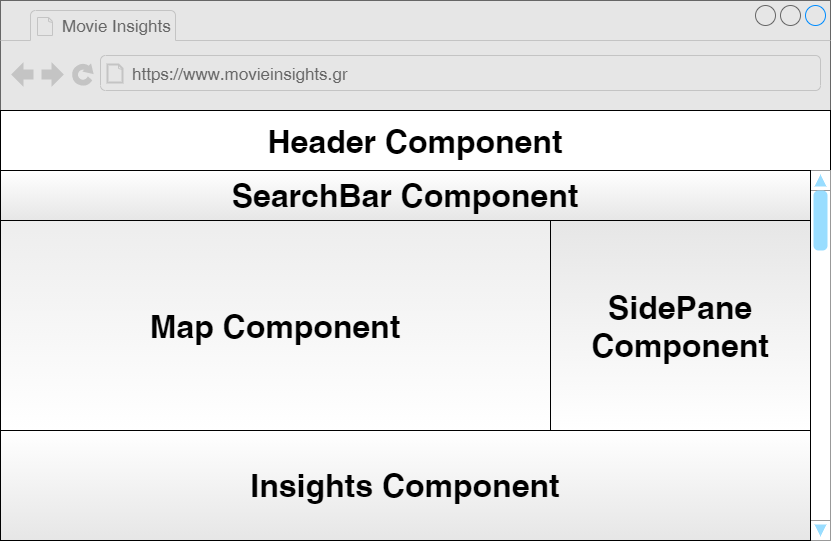
\includegraphics[width=145mm]{Chapters/5 - Architecture/Client/Images/dashboard_struct.png}
  \caption{Βασική διάταξη Web εφαρμογής}
  \label{wire:dashboard}
\end{figure}

Το Dashboard Module ορίζει το δικό του Router που αποτελείται από ένα Route /app/* και ένα RedirectRoute από το κεντρικό Route / στο /app το οποίο είναι η κεντρική σελίδα καθώς δεν χρειάζεται κάτι σύνθετο. 

Ο τρόπος που λειτουργεί είναι ο εξής. Είναι επιλεγμένη για παράδειγμα μια κατηγορία "Στοιχεία για την χώρα Ελλάδα".
Σε αυτήν την κατηγορία στα δεδομένα υπάρχουν οι πιο δημοφιλείς ηθοποιοί, παραγωγοί, σκηνοθέτες, συγγραφείς που έχουν συμμετάσχει σε ταινίες που είτε η παρήγαγε η Ελλάδα είτε η Ελλάδα ήταν χώρα συμπαραγωγής. Αναφέρει επίσης την πιο δημοφιλή εταιρία παραγωγής που συνεργάστηκε η Ελλάδα αλλά και την πιο δημοφιλή χώρα συμπαραγωγής και είδος ταινίας. Επιπρόσθετα αναφέρει τα μέσα και συνολικά έσοδα/έξοδα καθώς και το καθαρό κέρδος. Όλα αυτά τα στοιχεία υπάρχουν επίσης και ανά χρόνο, για όσα χρόνια υπάρχουν στην βάση δεδομένων για την Ελλάδα. Όλες οι κατηγορίες λειτουργούν με τον ίδιο τρόπο με την εξαίρεση της κατηγορίας ανά άτομο. Που εκεί εκτός από την επιλογή χρόνου, υπάρχει και η επιλογή ρόλου, με διαθέσιμους ρόλους: ηθοποιός, σκηνοθέτης, συγγραφέας και παραγωγός. Για τα άτομα υπάρχουν συγκεντρωτικά στοιχεία μόνο ανά ρόλο και όχι συνολικά, καθώς είναι διαφορετικά τα δεδομένα. Πάραυτα όλα τα στοιχεία ανά ρόλο υπάρχουν και ανά χρόνο.

Το Dashboard Module περιέχει μόνο ένα Component το ΜΙDashboard Component. Όλα τα δεδομένα που υπολογίζονται μέσα από το Dashboard Module στέλνονται απευθείας στο ΜΙDashboard Component.

Μέσω των Component που δηλώνονται και δομείται όλη η εφαρμογή καθίσταται εφικτή η πλοήγηση σε όλο το εύρος των δεδομένων της εφαρμογής. Ενώ θα μπορούσε σε κάθε Component, που επηρεάζει τα δεδομένα που εμφανίζονται, να υλοποιηθεί η λογική της αλλαγής των δεδομένων, προτιμήθηκε όλα αυτά τα Component απλά να αλλάζουν την διεύθυνση στην γραμμή διεύθυνσης του Browser και με βάση την διεύθυνση που άλλαξε χωρίς να γίνεται ανακατεύθυνση το Dashboard Module καταλαβαίνει τι χρειάζεται να αλλάξει, αλλάζει τα δεδομένα μέσω του Redux State Manager, και ύστερα στέλνει τα δεδομένα σε όλα τα επιμέρους Components για να αλλάξουν. Ενώ ακούγεται πιο σύνθετη τεχνική, χρησιμοποιήθηκε για την ευκολία διαχείρισης και συντήρησης του κώδικα, καθώς στην άλλη περίπτωση θα έπρεπε σε περίπτωση αλλαγής του κώδικα εμφάνισης των δεδομένων, να πραγματοποιηθούν αλλαγές σε κάθε Component που άλλαζε δεδομένα. Ενώ με αυτήν την υλοποίηση τα πάντα βρίσκονται σε ένα μέρος. Ένας ακόμα σημαντικός λόγος που προτιμήθηκε η συγκεκριμένη τεχνική είναι η προσβασιμότητα στα δεδομένα αυτά. Λόγω της φύσης της αρχιτεκτονικής της εφαρμογής και όντας SPA, υπάρχει ουσιαστικά μόνο μια αληθινή σελίδα που είναι προσβάσιμη από έναν Browser. Αυτή είναι η index.html που είναι ένα αρχείο HTML το οποίο φορτώνει όλον τον κώδικα της εφαρμογής. Χωρίς την αλλαγή της διεύθυνσης, ένας χρήστης θα έπρεπε να μπει στην αρχική σελίδα και να εκτελέσει κάποιες ενέργειες έτσι ώστε να φτάσει στο ίδιο σημείο που βρισκόταν πριν. Με την αλλαγή της διεύθυνσης όμως, όχι μόνο μπορεί να επανέλθει στο σημείο στο οποίο βρισκόταν αλλά μπορεί και να μοιραστεί τον σύνδεσμο με κάποιον άλλον χρήστη και να κοιτάνε τα ίδια δεδομένα. 

Το Dashboard Module λοιπόν παρακολουθεί τις αλλαγές διευθύνσεων που γίνονται μετά την βασική διεύθυνση /app/ και με την χρήση κάποιον βοηθητικών συναρτήσεων αλλάζει τα δεδομένα όπως φαίνεται στον κώδικα \ref{code:urlIntercept}.

\begin{figure}[h]
    \begin{TypeScriptcode}
handleViewChange = () => {
    const path = this.props.location.pathname;
    if (this.state.path !== path || !this.state.pathHandled) {
      if (!this.state.pathHandled) {
        let pathMatch: match;
        if ((pathMatch = matchPath(path, "/app/:entity(country|company|genre)/:id-:name/:year(\\d{4})?"))) {
          this.handleGenericChange(pathMatch.params['entity'], +pathMatch.params['id'], +pathMatch.params['year']);
        } else if ((pathMatch = matchPath(path, "/app/person/:id-:name/:role([A-z]+)?/:year(\\d{4})?"))) {
          this.handlePersonChange(+pathMatch.params['id'], +pathMatch.params['year'], pathMatch.params['role']);
        } else if ((pathMatch = matchPath(path, "/app/:general(general)?/:year(\\d{4})?"))) {
          this.handleGeneralChange(+pathMatch.params['year']);
        }
        this.scrollElement();
        if (this.state.path !== path)
          this.setState({path});
      }
      if (this.state.path !== path) {
        this.setState({pathHandled: false});
      }
    }
}
    \end{TypeScriptcode}
    \caption{Αλγόριθμος παρακολούθησης αλλαγής στην γραμμή διευθύνσεων ενός Browser.}
   \label{code:urlIntercept}
\end{figure}

Η αλλαγή της διεύθυνσης στην γραμμή διευθύνσεων του Browser, δημιουργείται από μια βοηθητική συνάρτηση όπως φαίνεται στον κώδικα \ref{code:urlBuilder}. Με αυτόν τον τρόπο όλα τα Components που έχουν ως σκοπό την αλλαγή των δεδομένων μπορούν να αλλάξουν εύκολα την διεύθυνση χρησιμοποιώντας αυτήν την συνάρτηση, και αν αλλάξει ποτέ η δομή της διεύθυνσης η αλλαγή θα γίνει μόνο μέσα σε αυτήν την συνάρτηση διευκολύνοντας παράλληλα την συντήρηση και την αντιμετώπιση προβλημάτων του κώδικα.

\begin{figure}[h]
    \begin{TypeScriptcode}
function |$\textbf{generateNavigationLink}$|(entity?: BaseNamedEntity, role?: CreditRole, year?: number, entityType?: EntityType) {
  let type = undefined;
  if (entity) {
    if (entityType) {
      type = entityType.toLowerCase();
    } else if (isMovie(entity)) {
      type = 'movie';
    } else if (isPerson(entity)) {
      type = 'person';
    } else if (isCompany(entity)) {
      type = 'company';
    } else if (isCountry(entity)) {
      type = 'country';
    } else if (isGenre(entity)) {
      type = 'genre';
    }
  } else if (year) {
    type = 'general';
  }
  return `/app${type ? `/${type}` : ''}${entity ? `/${entity.id}-${normalizeText(entity.name)}` : ''}${role && type === 'person' ? `/${role}` : ''}${year ? `/${year}` : ''}`;
}
    \end{TypeScriptcode}
    \caption{Αλγόριθμος δημιουργίας διεύθυνσης αλλαγής δεδομένων.}
   \label{code:urlBuilder}
\end{figure}

Το Redux State Manager χρησιμοποιήθηκε για 2 λόγους. Προσφέρει μια εύκολη διεπαφή που βασίζεται στο Immutability των δεδομένων συμβάλλοντας δραστικά στην μείωση των Side Effects, αλλά επίσης χρησιμοποιήθηκε σαν ένα Facade για την απόκτηση των δεδομένων από την υπηρεσία.

Γνωρίζοντάς ότι οποιαδήποτε ενέργεια εμπεριέχει κάποιου είδους επικοινωνία με μια εξωτερική υπηρεσία αυξάνει σημαντικά τον χρόνο της διεκπεραίωσης της, και έχοντας σαν δεδομένο ότι η JavaScript που τρέχει μέσα σε έναν Browser τρέχει σε ένα και μοναδικό νήμα (Thread), η εμπειρία του χρήστη θα ήταν πολύ άσχημη όταν θα ζητούσε νέα δεδομένα από τον Server, καθώς η Web Εφαρμογή θα ήταν μη αποκρίσιμη για αρκετό διάστημα μέχρι την απόκτηση των δεδομένων και την εμφάνιση τους. Για αυτόν τον λόγο χρησιμοποιήθηκε ένα πρόσθετο στο Redux Fraemwork, που επιτρέπει την ασύγχρονη απόκτηση δεδομένων και την αποθήκευση τους στο κεντρικό State της εφαρμογής. Όλα τα Components που εξαρτιούνται από αυτό το Global State, όταν αλλάξει θα αλλάξουν και αυτά τα δεδομένα που εμφανίζουν.

Όπως προαναφέρθηκε το Dashboard Component περιέχει 4 σημαντικά Component που εμφανίζουν όλα τα απαραίτητα δεδομένα.

\subsubsection{SearchBar Component}
Το πρώτο Component μέσα στο MIDashboard Component είναι η γραμμή αναζήτησης, MISearchBar Component. Το MISearchBar Component δεν προσφέρει την δυνατότητα γενικής αναζήτησης αλλά μόνο την δυνατότητα επιλογής ενός αποτελέσματος απο τις προτάσεις της μηχανής αναζήτησης. Οι προτάσεις δημιουργούνται απο την μηχανή αναζήτησης μέσο του Server όπως προαναφέρθηκε νωρίτερα κάθε φορά που ο χρήστης γράφει οποιοδήποτε γράμμα στην μπάρα αναζήτησης όπως φαίνεται στον κώδικα \ref{code:searchbar_suggestion}.

\begin{figure}[H]
    \begin{TypeScriptcode}
async function getSuggestions(value: string): Promise<ACResult[]> {
    const results: AutoComplete = (await Service.search(value)).data;
    return results._
      .map(result => {
        result.e.forEach(e => {
          e.i = result.i
        })
        return result;
      })
      .filter(result => result.e.length > 0);
}
    \end{TypeScriptcode}
    \caption{Αλγόριθμος ανάκτησης προτάσεων αποτελεσμάτων μηχανής αναζήτησης}
   \label{code:searchbar_suggestion}
\end{figure}

Οι προτάσεις της μηχανής αναζήτησης εμφανίζονται με μια μικρή εικόνα στα αριστερά και το κείμενο του αποτελέσματος ακριβώς από διπλά. Ανάλογα με το κείμενο της αναζήτησης που έγραψε ο χρήστης προσπαθεί να υπογραμμίσει με μπλε χρώμα τα γράμματα που βρέθηκαν στα αποτελέσματα όπως φαίνεται στην εικόνα \ref{layout:misearchbar}.
\begin{figure}[H]
  \centering
  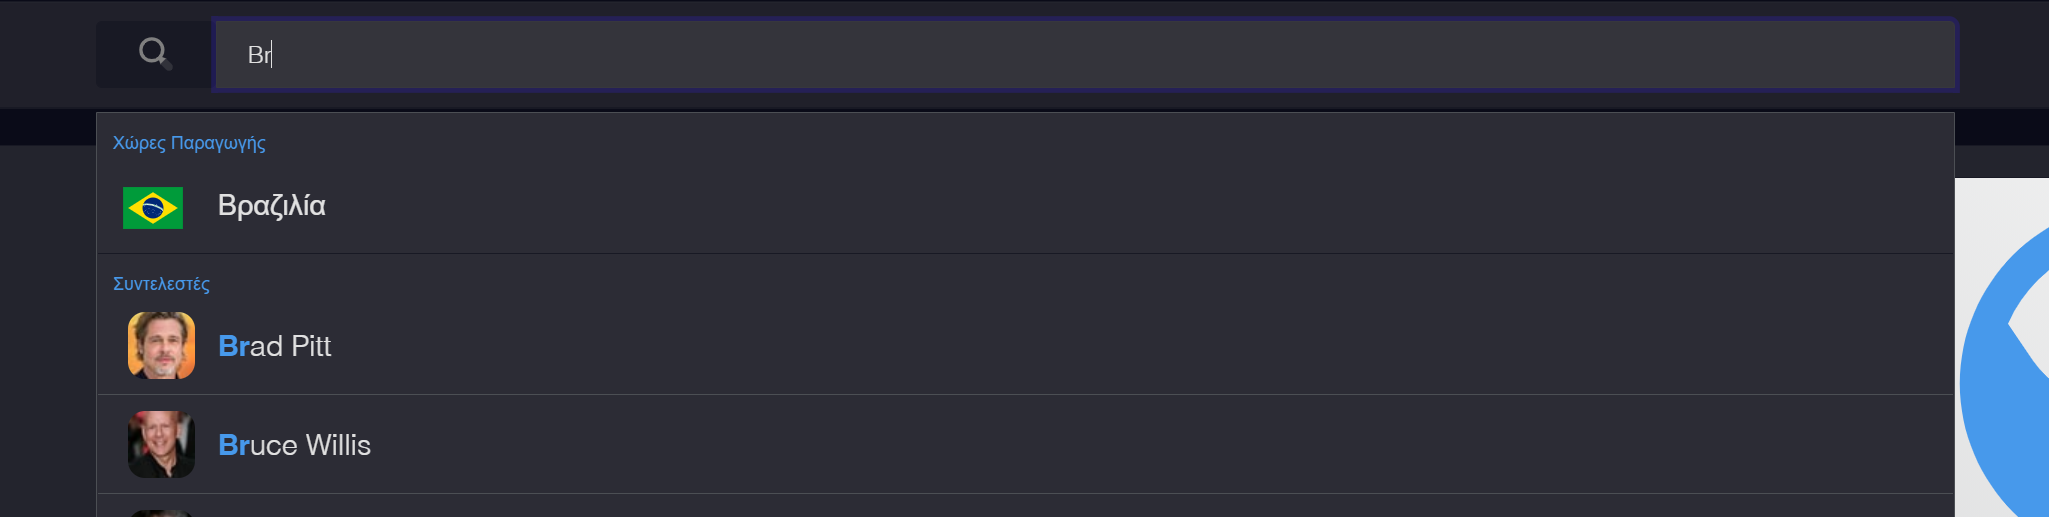
\includegraphics[width=145mm]{Chapters/5 - Architecture/Client/Images/misearchbar_results.png}
  \caption{MISearchBar Component}
  \label{layout:misearchbar}
\end{figure}
Οταν επιλεγεί ενα απο τα προτεινόμενα αποτελέσματα η μπάρα αναζήτησης σβήνει και αλλάζει η διεύθυνση όπως φαίνεται στον κώδικα \ref{code:searchbar_urlchange}

\begin{figure}[H]
    \begin{TypeScriptcode}
private onSearch = (val: ACEntity) => {
  this.props.history.push(AppUtils.|\textbf{generateNavigationLink}|(val, null, null, val.i));
}
    \end{TypeScriptcode}
    \caption{Αλγόριθμος αλλαγής διεύθυνσης απο το MISearchBar Component}
   \label{code:searchbar_urlchange}
\end{figure}

\subsubsection{MapComponent}
Το δεύτερο είναι το Map Component και είναι ένα Component το οποίο προσφέρει ένα προ-ρυθμισμένο Chart από την βιβλιοθήκη Highcharts Highmaps και προσφέρει μια εύκολη διεπαφή για την αλληλεπίδραση και εμφάνιση δεδομένων σε αυτόν τον χάρτη όπως φαίνεται στο σχήμα \ref{layout:mapcomponent}. Κάθε φορά που ο δείκτης του ποντικιού περνάει πάνω απο μια χώρα εμφανίζεται ενα tooltip που γράφει το όνομα της χώρας και σε πόσες ταινίες έχει συμμετάσχει αυτή η χώρα. Όταν πατηθεί μια χώρα θα επιλεγεί εκτός αν ήταν ήδη επιλεγμένη που τότε θα σταματήσει να είναι επιλεγμένη και θα αλλάξει η διεύθυνση όπως φαίνεται στον κώδικα στο σχήμα \ref{code:map_urlchanger}.
\begin{figure}[H]
  \centering
  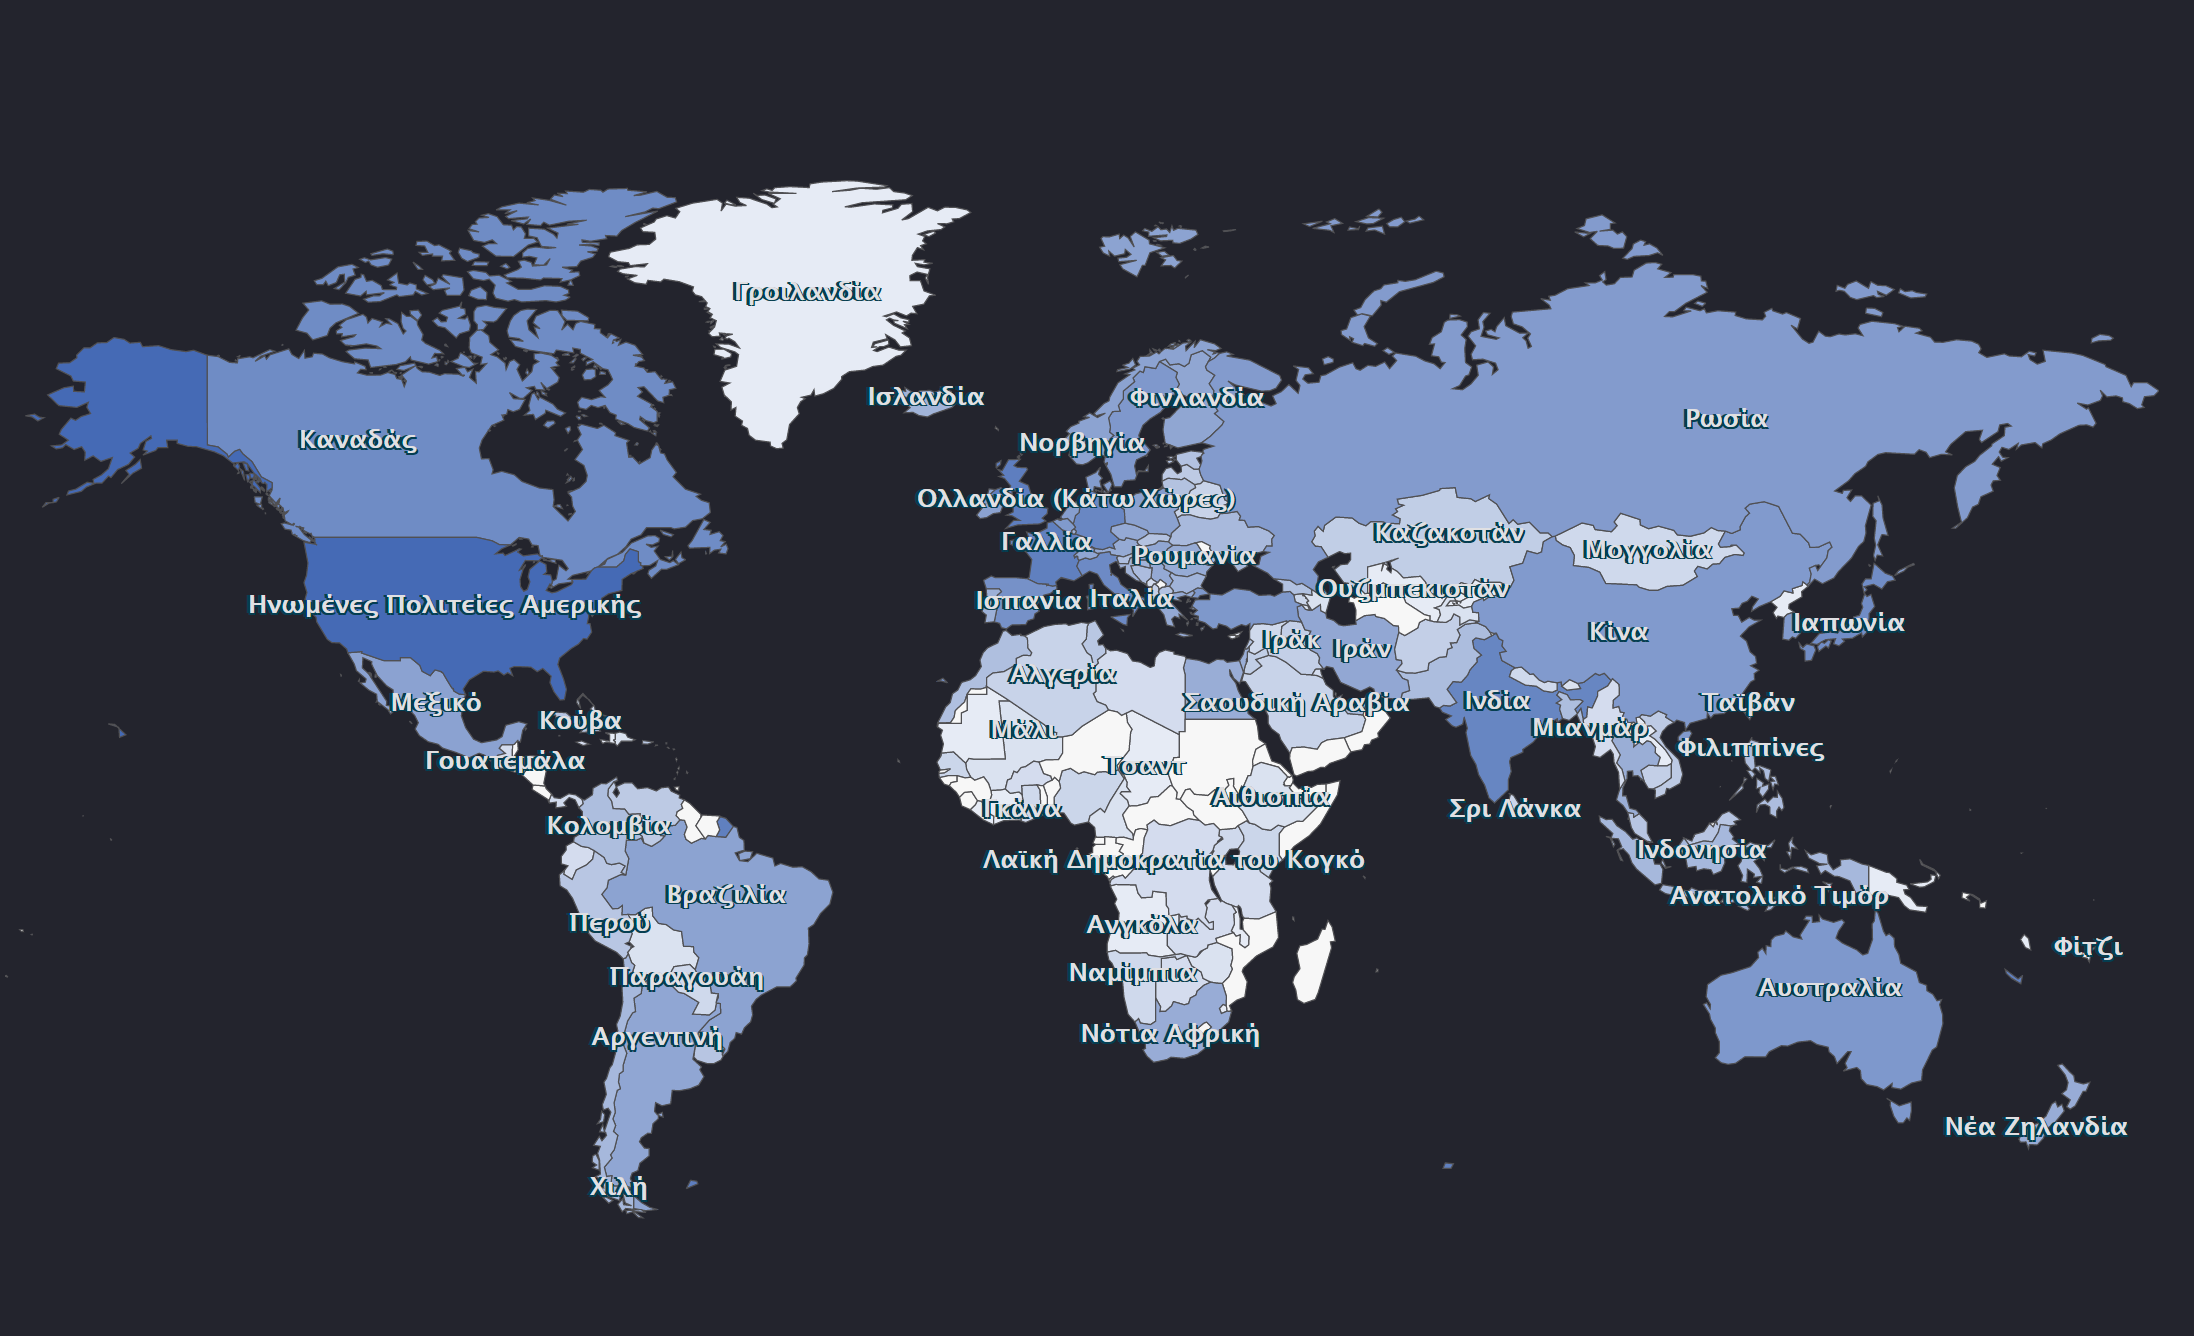
\includegraphics[width=140mm]{Chapters/5 - Architecture/Client/Images/world_map.PNG}
  \caption{Map Component}
  \label{layout:mapcomponent}
\end{figure}

\begin{figure}[H]
    \begin{TypeScriptcode}
countrySelected = (data: ICountryData) => {
  this.props.history.push(AppUtils.|$\textbf{generateNavigationLink}$|({id: data._id, name: data.name, iso31661: data.iso31661, movies: []} as IProductionCountry))
}
countryUnselected = () => {
  this.props.history.push(`/app`)
}
    \end{TypeScriptcode}
    \caption{Αλγόριθμος αλλαγής διεύθυνσης απο το Map Component.}
   \label{code:map_urlchanger}
\end{figure}
\subsubsection{MISidePane Component}
Το ΜΙSidepane Component είναι το τρίτο Component μέσα στο MIDashboard Component και περιέχει το όνομα της κατηγορίας και μια φωτογραφία αν υπάρχει
για παράδειγμα αν είναι η κατηγορία ανά ηθοποιό και ο ηθοποιός ονομαζόταν Νικόλαος Μαυρόπουλος θα εμφάνιζε αυτό το άτομο και την φωτογραφία του αν υπάρχει στην βάση δεδομένων. Περιέχει επίσης ένα Component για την δυνατότητα φιλτραρίσματος των αποτελεσμάτων ανα χρόνο, το MIYearPicker Component, και παρακάτω 4 ίδια Component τύπου MIChartCard για εμφάνιση δεδομένων και γραφημάτων συνδυαστικά. Επί το πλείστον η διάταξη του MISidePane Component παραμένει σταθερή με εξαίρεση την κατηγορία "ανά άτομο" που προστίθεται ένα ακόμα Component το MIRolePicker που δίνει την δυνατότητα φιλτραρίσματος του ρόλου του ατόμου δηλαδή ηθοποιό, σκηνοθέτη, συγγραφέα και παραγωγό.

\input{Chapters/5 - Architecture/Client/SidePaneComponent/MIChartCard}
\input{Chapters/5 - Architecture/Client/SidePaneComponent/MIYearPicker}
\input{Chapters/5 - Architecture/Client/SidePaneComponent/MIRolePicker}



\subsubsection{MIInsightsPanel Component}
Το MIInsightsPanel Component είναι το τέταρτο και τελευταίο Component που βρίσκεται μέσα στο MIDashboard Component.
Περιέχει πολλά Component ίδιου τύπου MICard Component. Το κάθε MICard Component είναι μια "κάρτα" που εμφανίζει ένα στοιχείο για ένα άτομο, μια ταινία, μια εταιρία παραγωγής, μια χώρα παραγωγής η ένα είδος ταινίας. Για παράδειγμα αν μια κάρτα για μια ταινία με τα μεγαλύτερα έσοδα θα εμφανιζόταν όπως στο σχήμα \ref{layout:micard_revenue}.

\begin{figure}[h]
  \centering
  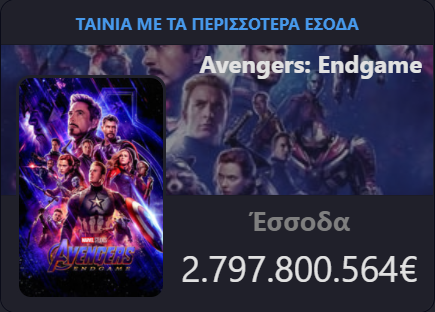
\includegraphics[width=50mm]{Chapters/5 - Architecture/Client/Images/micard_revenue.png}
  \caption{MICard Component}
  \label{layout:micard_revenue}
\end{figure}

\input{Chapters/5 - Architecture/Client/InsightsComponent/MICard}
\input{Chapters/5 - Architecture/Client/InsightsComponent/MIMovieModal}
\subsection{Admin Module}
Το Admin Module είναι ένα σύνολο λειτουργιών που επιτρέπει έναν διαχειριστή να διαχειρίζεται με ευκολία την εφαρμογή. Στην παρούσα υλοποίηση το Admin Module έχει 2 διαφορετικές σελίδες - Components, το Κέντρο Ελέγχου και το Κέντρο Διαχείρισης Καταγραφών. Για να αποκτήσει πρόσβαση ένας χρήστης στις λειτουργίες του Admin Module, πρέπει να έχει κάνει Login και να είναι εξουσιοδοτημένος με τον ρόλο ADMIN, διαχειριστή. 

Το Κέντρο Ελέγχου είναι μια σελίδα που επιτρέπει την παρακολούθηση της κατάστασης της υγείας της εφαρμογής, προσφέρει στατιστικά των υπηρεσιών αλλά και του λειτουργικού που τρέχει η εφαρμογή αλλα παράλληλα προσφέρει και διαγνωστικά για να γνωρίζει ο διαχειριστής τι γίνεται ανά πάσα στιγμή στην εφαρμογή αυτήν όπως φαίνεται στις εικόνες \ref{layout:admin_cc_1} και \ref{layout:admin_cc_2}. 

Αποτελείται από πολλά διαφορετικά Components τα οποία ενημερώνονται ανάλογα με τον τύπο των δεδομένων που προσφέρουν ανά μισό, δύο και ανά πέντε δευτερόλεπτα με την χρήση WebSockets μέσο του Spring Boot Actuator έτσι ώστε η εικόνα που βλέπει ο διαχειριστής να αντικατοπτρίζει πάντα την κατάσταση της εφαρμογής εκείνη την χρονική στιγμή.

Το Κέντρο Διαχείρισής Καταγραφών είναι στην ουσία ένας διαδραστικός πίνακας που επιτρέπει στον διαχειριστή να αλλάζει τα επίπεδα καταγραφής διάφορων υπηρεσιών μέσα στον Server. Τα επίπεδα καταγραφής ορίζουν τι πληροφορίες θα δίνει η κάθε υπηρεσία. Το επίπεδο καταγραφής ERROR για παράδειγμα καταγράφει μόνο τα μηνύματα σφαλμάτων στο αρχείο καταγραφής της υπηρεσίας, ενώ το επίπεδο καταγραφής WARNING καταγράφει και τα μηνύματα σφαλμάτων αλλά και τα μηνύματα προειδοποιήσεων. Αυτό είναι πολύ χρήσιμο όταν χρησιμοποιείται σε συνδυασμό με μια υπηρεσία διαχείρισης καταγραφών όπως η Logstash για παράδειγμα. Με αυτόν τον τρόπο ο διαχειριστής δεν χρειάζεται να έχει φυσική πρόσβαση στο μηχάνημα που τρέχει την εφαρμογή για να μπορεί να δει τα αρχεία καταγραφής παρά μόνο να μπει στην υπηρεσία διαχείρισης καταγραφών και να βρει ότι χρειάζεται από εκεί.

Ο πίνακας του Κέντρου Διαχείρισής Καταγραφών φαίνεται στην εικόνα \ref{layout:admin_l}. Η συγκεκριμένη εικόνα τραβήχτηκε κατά την ανάπτυξη της εφαρμογής και δείχνει ότι το κεντρικό επίπεδο καταγραφών ROOT είναι ορισμένο στο DEBUG που σημαίνει ότι καταγράφει ακόμα και μηνύματα διαγνωστικών με κάποιες εξαιρέσεις που έχουν οριστεί σε επίπεδο WARNING για να μην υπερφορτώσουν τα αρχεία καταγραφής με περιττές πληροφορίες.

\begin{figure}[H]
  \centering
  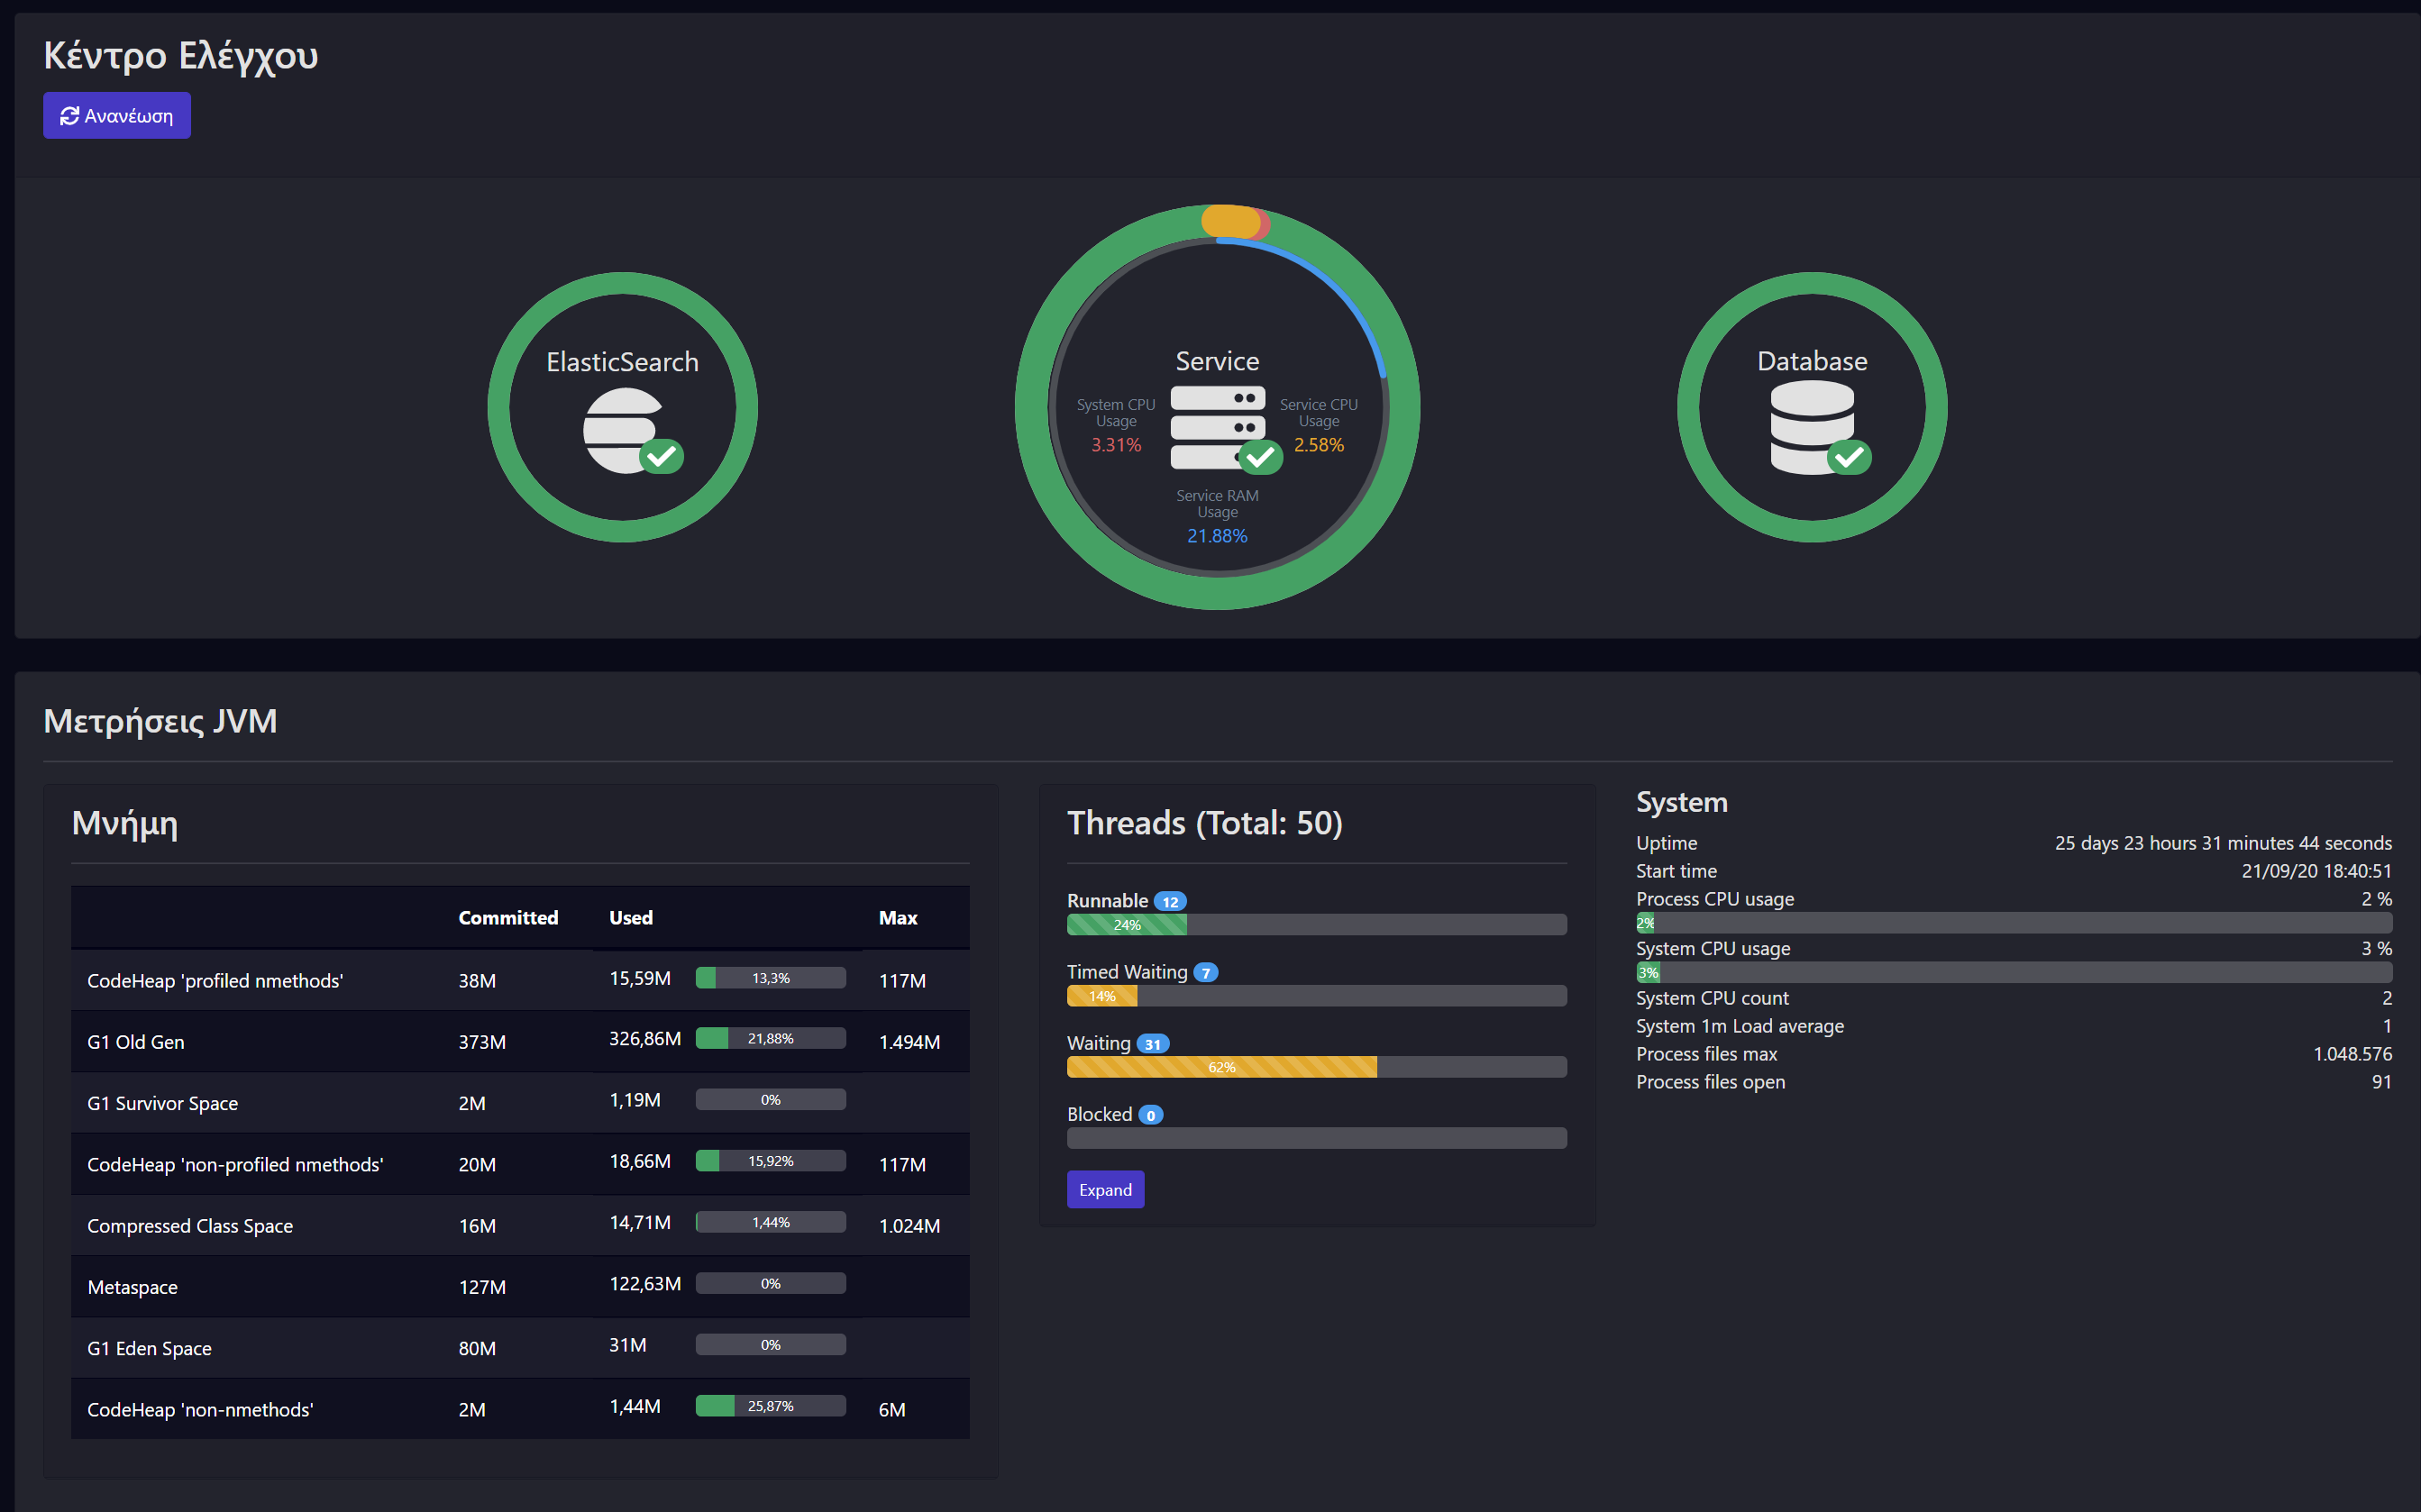
\includegraphics[width=145mm]{Chapters/5 - Architecture/Client/Images/admin_control_center.png}
  \caption{Κέντρο Ελέγχου}
  \label{layout:admin_cc_1}
\end{figure}
\begin{figure}[H]
  \centering
  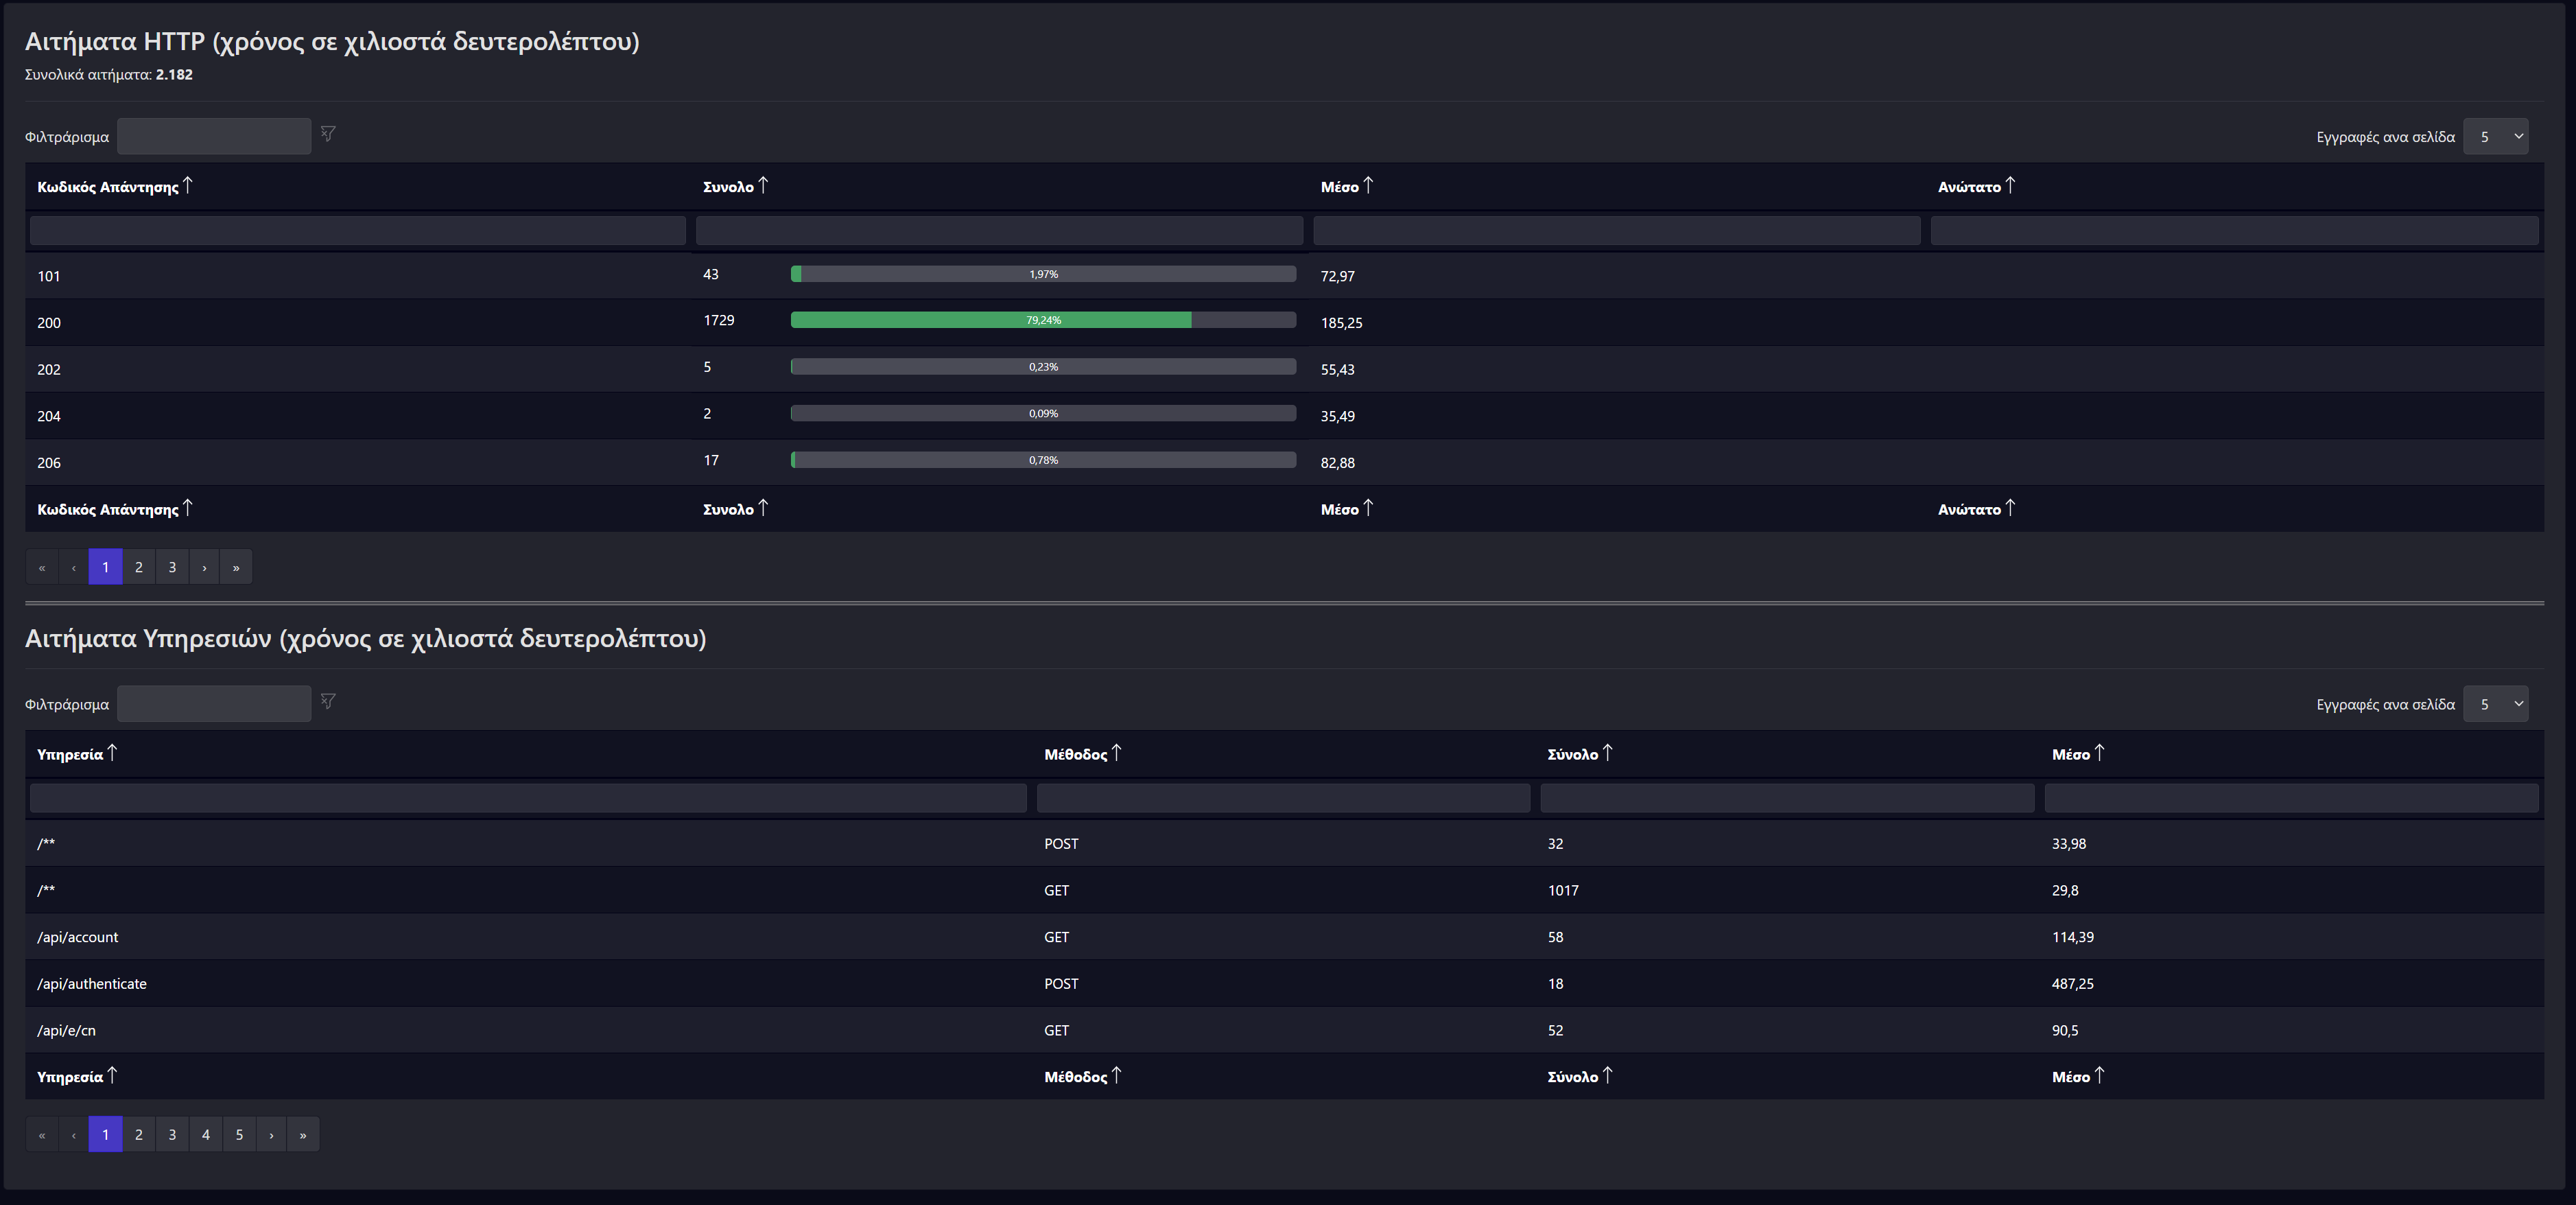
\includegraphics[width=145mm]{Chapters/5 - Architecture/Client/Images/admin_control_center_2.png}
  \caption{Κέντρου Ελέγχου - συνέχεια}
  \label{layout:admin_cc_2}
\end{figure}
\begin{figure}[H]
  \centering
  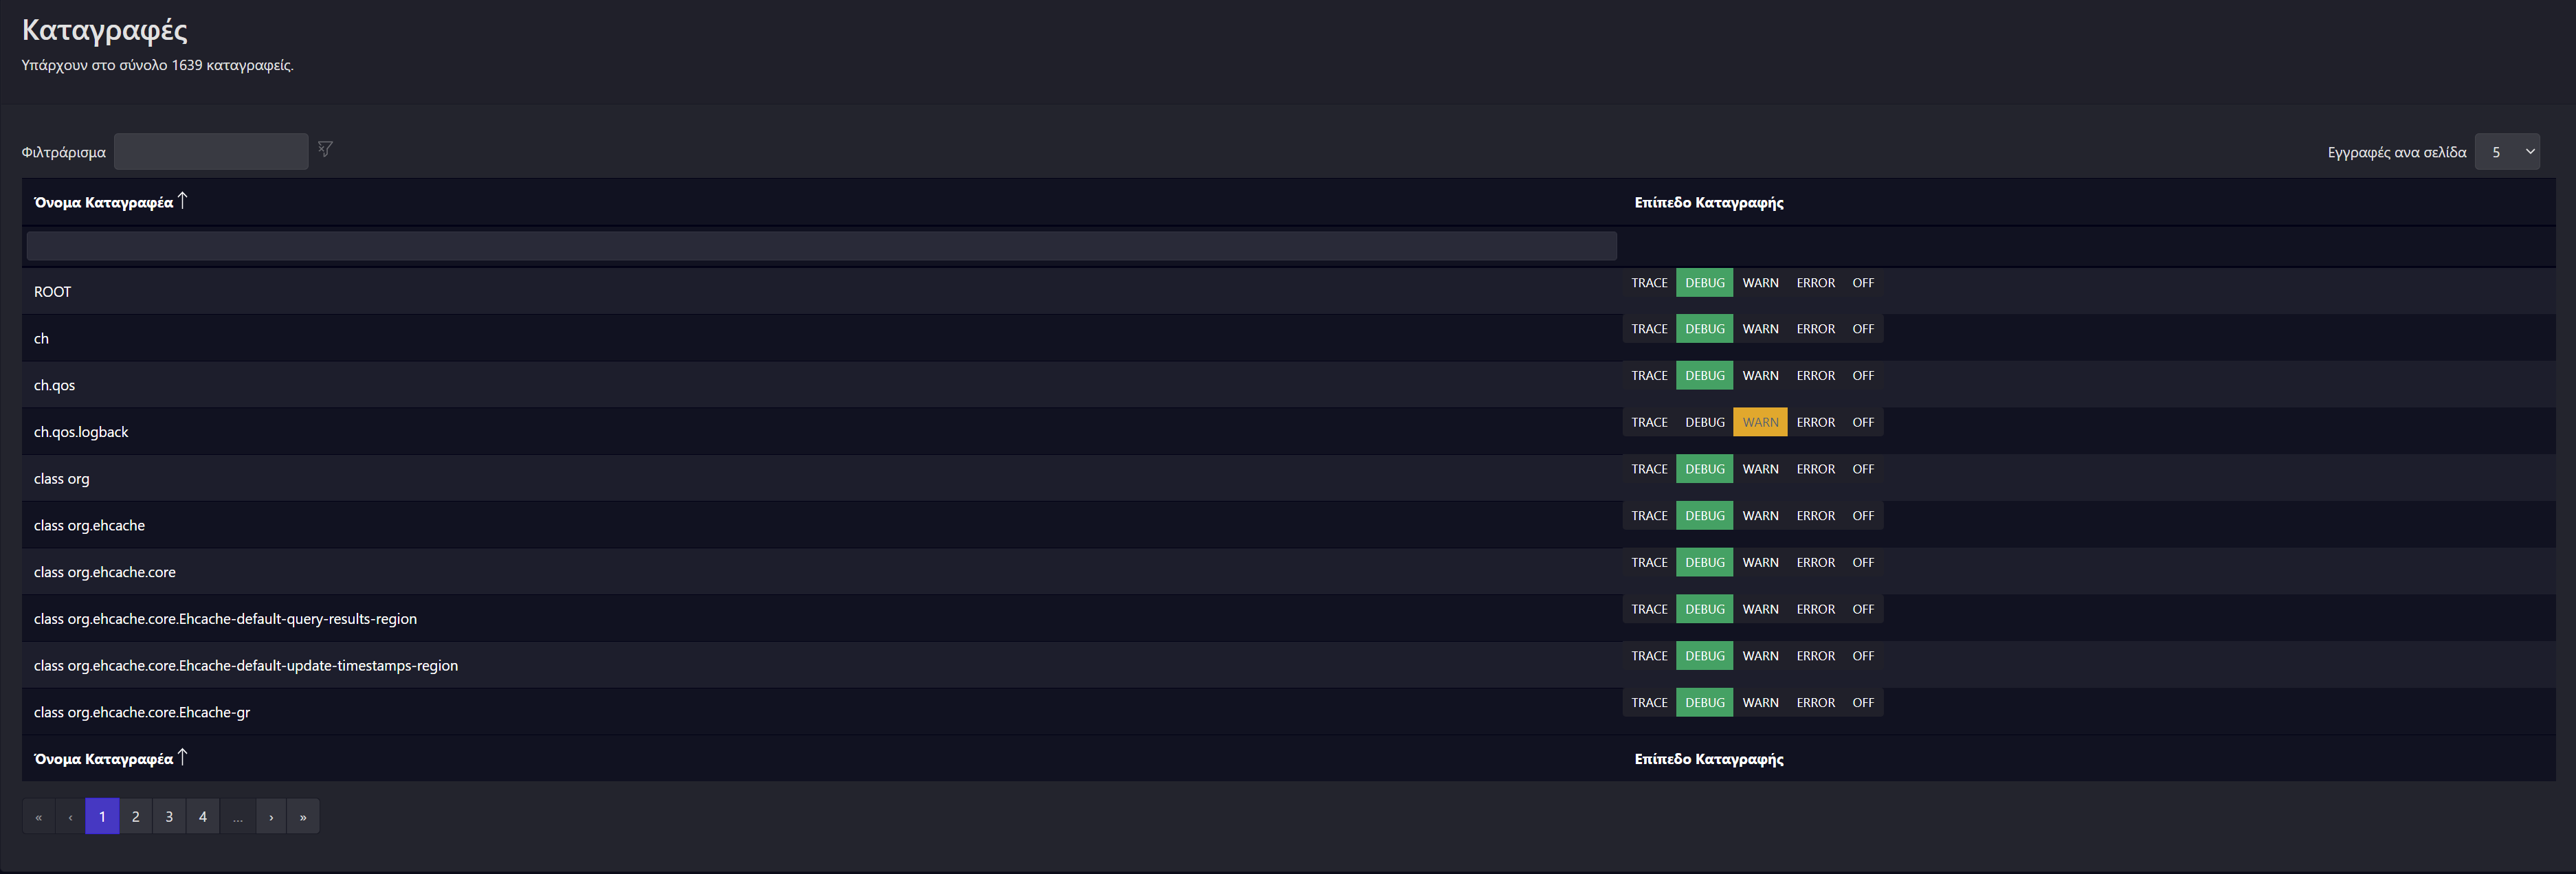
\includegraphics[width=145mm]{Chapters/5 - Architecture/Client/Images/admin_l.png}
  \caption{Κέντρο Διαχείρισής Καταγραφών}
  \label{layout:admin_l}
\end{figure}